% Generated by Sphinx.
\def\sphinxdocclass{report}
\documentclass[letterpaper,10pt,english]{sphinxmanual}
\usepackage[utf8]{inputenc}
\DeclareUnicodeCharacter{00A0}{\nobreakspace}
\usepackage[T1]{fontenc}
\usepackage{babel}
\usepackage{times}
\usepackage[Bjarne]{fncychap}
\usepackage{longtable}
\usepackage{sphinx}
\usepackage{multirow}


\title{AOSB Manual}
\date{May 01, 2014}
\release{alpha}
\author{Philipp Boeing}
\newcommand{\sphinxlogo}{}
\renewcommand{\releasename}{Release}
\makeindex

\makeatletter
\def\PYG@reset{\let\PYG@it=\relax \let\PYG@bf=\relax%
    \let\PYG@ul=\relax \let\PYG@tc=\relax%
    \let\PYG@bc=\relax \let\PYG@ff=\relax}
\def\PYG@tok#1{\csname PYG@tok@#1\endcsname}
\def\PYG@toks#1+{\ifx\relax#1\empty\else%
    \PYG@tok{#1}\expandafter\PYG@toks\fi}
\def\PYG@do#1{\PYG@bc{\PYG@tc{\PYG@ul{%
    \PYG@it{\PYG@bf{\PYG@ff{#1}}}}}}}
\def\PYG#1#2{\PYG@reset\PYG@toks#1+\relax+\PYG@do{#2}}

\def\PYG@tok@gd{\def\PYG@tc##1{\textcolor[rgb]{0.63,0.00,0.00}{##1}}}
\def\PYG@tok@gu{\let\PYG@bf=\textbf\def\PYG@tc##1{\textcolor[rgb]{0.50,0.00,0.50}{##1}}}
\def\PYG@tok@gt{\def\PYG@tc##1{\textcolor[rgb]{0.00,0.25,0.82}{##1}}}
\def\PYG@tok@gs{\let\PYG@bf=\textbf}
\def\PYG@tok@gr{\def\PYG@tc##1{\textcolor[rgb]{1.00,0.00,0.00}{##1}}}
\def\PYG@tok@cm{\let\PYG@it=\textit\def\PYG@tc##1{\textcolor[rgb]{0.25,0.50,0.56}{##1}}}
\def\PYG@tok@vg{\def\PYG@tc##1{\textcolor[rgb]{0.73,0.38,0.84}{##1}}}
\def\PYG@tok@m{\def\PYG@tc##1{\textcolor[rgb]{0.13,0.50,0.31}{##1}}}
\def\PYG@tok@mh{\def\PYG@tc##1{\textcolor[rgb]{0.13,0.50,0.31}{##1}}}
\def\PYG@tok@cs{\def\PYG@tc##1{\textcolor[rgb]{0.25,0.50,0.56}{##1}}\def\PYG@bc##1{\colorbox[rgb]{1.00,0.94,0.94}{##1}}}
\def\PYG@tok@ge{\let\PYG@it=\textit}
\def\PYG@tok@vc{\def\PYG@tc##1{\textcolor[rgb]{0.73,0.38,0.84}{##1}}}
\def\PYG@tok@il{\def\PYG@tc##1{\textcolor[rgb]{0.13,0.50,0.31}{##1}}}
\def\PYG@tok@go{\def\PYG@tc##1{\textcolor[rgb]{0.19,0.19,0.19}{##1}}}
\def\PYG@tok@cp{\def\PYG@tc##1{\textcolor[rgb]{0.00,0.44,0.13}{##1}}}
\def\PYG@tok@gi{\def\PYG@tc##1{\textcolor[rgb]{0.00,0.63,0.00}{##1}}}
\def\PYG@tok@gh{\let\PYG@bf=\textbf\def\PYG@tc##1{\textcolor[rgb]{0.00,0.00,0.50}{##1}}}
\def\PYG@tok@ni{\let\PYG@bf=\textbf\def\PYG@tc##1{\textcolor[rgb]{0.84,0.33,0.22}{##1}}}
\def\PYG@tok@nl{\let\PYG@bf=\textbf\def\PYG@tc##1{\textcolor[rgb]{0.00,0.13,0.44}{##1}}}
\def\PYG@tok@nn{\let\PYG@bf=\textbf\def\PYG@tc##1{\textcolor[rgb]{0.05,0.52,0.71}{##1}}}
\def\PYG@tok@no{\def\PYG@tc##1{\textcolor[rgb]{0.38,0.68,0.84}{##1}}}
\def\PYG@tok@na{\def\PYG@tc##1{\textcolor[rgb]{0.25,0.44,0.63}{##1}}}
\def\PYG@tok@nb{\def\PYG@tc##1{\textcolor[rgb]{0.00,0.44,0.13}{##1}}}
\def\PYG@tok@nc{\let\PYG@bf=\textbf\def\PYG@tc##1{\textcolor[rgb]{0.05,0.52,0.71}{##1}}}
\def\PYG@tok@nd{\let\PYG@bf=\textbf\def\PYG@tc##1{\textcolor[rgb]{0.33,0.33,0.33}{##1}}}
\def\PYG@tok@ne{\def\PYG@tc##1{\textcolor[rgb]{0.00,0.44,0.13}{##1}}}
\def\PYG@tok@nf{\def\PYG@tc##1{\textcolor[rgb]{0.02,0.16,0.49}{##1}}}
\def\PYG@tok@si{\let\PYG@it=\textit\def\PYG@tc##1{\textcolor[rgb]{0.44,0.63,0.82}{##1}}}
\def\PYG@tok@s2{\def\PYG@tc##1{\textcolor[rgb]{0.25,0.44,0.63}{##1}}}
\def\PYG@tok@vi{\def\PYG@tc##1{\textcolor[rgb]{0.73,0.38,0.84}{##1}}}
\def\PYG@tok@nt{\let\PYG@bf=\textbf\def\PYG@tc##1{\textcolor[rgb]{0.02,0.16,0.45}{##1}}}
\def\PYG@tok@nv{\def\PYG@tc##1{\textcolor[rgb]{0.73,0.38,0.84}{##1}}}
\def\PYG@tok@s1{\def\PYG@tc##1{\textcolor[rgb]{0.25,0.44,0.63}{##1}}}
\def\PYG@tok@gp{\let\PYG@bf=\textbf\def\PYG@tc##1{\textcolor[rgb]{0.78,0.36,0.04}{##1}}}
\def\PYG@tok@sh{\def\PYG@tc##1{\textcolor[rgb]{0.25,0.44,0.63}{##1}}}
\def\PYG@tok@ow{\let\PYG@bf=\textbf\def\PYG@tc##1{\textcolor[rgb]{0.00,0.44,0.13}{##1}}}
\def\PYG@tok@sx{\def\PYG@tc##1{\textcolor[rgb]{0.78,0.36,0.04}{##1}}}
\def\PYG@tok@bp{\def\PYG@tc##1{\textcolor[rgb]{0.00,0.44,0.13}{##1}}}
\def\PYG@tok@c1{\let\PYG@it=\textit\def\PYG@tc##1{\textcolor[rgb]{0.25,0.50,0.56}{##1}}}
\def\PYG@tok@kc{\let\PYG@bf=\textbf\def\PYG@tc##1{\textcolor[rgb]{0.00,0.44,0.13}{##1}}}
\def\PYG@tok@c{\let\PYG@it=\textit\def\PYG@tc##1{\textcolor[rgb]{0.25,0.50,0.56}{##1}}}
\def\PYG@tok@mf{\def\PYG@tc##1{\textcolor[rgb]{0.13,0.50,0.31}{##1}}}
\def\PYG@tok@err{\def\PYG@bc##1{\fcolorbox[rgb]{1.00,0.00,0.00}{1,1,1}{##1}}}
\def\PYG@tok@kd{\let\PYG@bf=\textbf\def\PYG@tc##1{\textcolor[rgb]{0.00,0.44,0.13}{##1}}}
\def\PYG@tok@ss{\def\PYG@tc##1{\textcolor[rgb]{0.32,0.47,0.09}{##1}}}
\def\PYG@tok@sr{\def\PYG@tc##1{\textcolor[rgb]{0.14,0.33,0.53}{##1}}}
\def\PYG@tok@mo{\def\PYG@tc##1{\textcolor[rgb]{0.13,0.50,0.31}{##1}}}
\def\PYG@tok@mi{\def\PYG@tc##1{\textcolor[rgb]{0.13,0.50,0.31}{##1}}}
\def\PYG@tok@kn{\let\PYG@bf=\textbf\def\PYG@tc##1{\textcolor[rgb]{0.00,0.44,0.13}{##1}}}
\def\PYG@tok@o{\def\PYG@tc##1{\textcolor[rgb]{0.40,0.40,0.40}{##1}}}
\def\PYG@tok@kr{\let\PYG@bf=\textbf\def\PYG@tc##1{\textcolor[rgb]{0.00,0.44,0.13}{##1}}}
\def\PYG@tok@s{\def\PYG@tc##1{\textcolor[rgb]{0.25,0.44,0.63}{##1}}}
\def\PYG@tok@kp{\def\PYG@tc##1{\textcolor[rgb]{0.00,0.44,0.13}{##1}}}
\def\PYG@tok@w{\def\PYG@tc##1{\textcolor[rgb]{0.73,0.73,0.73}{##1}}}
\def\PYG@tok@kt{\def\PYG@tc##1{\textcolor[rgb]{0.56,0.13,0.00}{##1}}}
\def\PYG@tok@sc{\def\PYG@tc##1{\textcolor[rgb]{0.25,0.44,0.63}{##1}}}
\def\PYG@tok@sb{\def\PYG@tc##1{\textcolor[rgb]{0.25,0.44,0.63}{##1}}}
\def\PYG@tok@k{\let\PYG@bf=\textbf\def\PYG@tc##1{\textcolor[rgb]{0.00,0.44,0.13}{##1}}}
\def\PYG@tok@se{\let\PYG@bf=\textbf\def\PYG@tc##1{\textcolor[rgb]{0.25,0.44,0.63}{##1}}}
\def\PYG@tok@sd{\let\PYG@it=\textit\def\PYG@tc##1{\textcolor[rgb]{0.25,0.44,0.63}{##1}}}

\def\PYGZbs{\char`\\}
\def\PYGZus{\char`\_}
\def\PYGZob{\char`\{}
\def\PYGZcb{\char`\}}
\def\PYGZca{\char`\^}
\def\PYGZsh{\char`\#}
\def\PYGZpc{\char`\%}
\def\PYGZdl{\char`\$}
\def\PYGZti{\char`\~}
% for compatibility with earlier versions
\def\PYGZat{@}
\def\PYGZlb{[}
\def\PYGZrb{]}
\makeatother

\begin{document}

\maketitle
\tableofcontents
\phantomsection\label{index::doc}


Contents:


\chapter{Tutorial}
\label{tutorial::doc}\label{tutorial:aosb-documentation}\label{tutorial:tutorial}

\section{Introduction}
\label{tutorial:introduction}
This tutorial will introduce the main constructs of the AOSB framework and
how to use them to build an aspect oriented synthetic biology design. However,
it is not written as an in-depth tutorial into thinking about synthetic biology
systems in terms of cross-cutting concern separation and aspect modularization.
It simply serves as an introduction to the AOSB language defined by the framework.


\section{Prerequisites}
\label{tutorial:prerequisites}
AOSB is a framework for Python 2.7. The tutorial assumes at least basic knowledge
of the Python programming language and object oriented programming as well as a
conceptual awareness of aspect oriented programming.

The AOSB package must also be added to the Python path.


\section{Hello World}
\label{tutorial:hello-world}
AOSB allows a genetic circuit, i.e. a synthetic biology ``program'' to be defined
and manipulated in Python. Let us start by creating a simple example. In an empty
Python file, first import the AOSB framework:

\begin{Verbatim}[commandchars=\\\{\}]
\PYG{k+kn}{from} \PYG{n+nn}{aosb} \PYG{k+kn}{import} \PYG{o}{*}
\end{Verbatim}

Next, we will define a simple genetic circuit expressing an undefined Protein:

\begin{Verbatim}[commandchars=\\\{\}]
\PYG{k}{class} \PYG{n+nc}{SimpleCircuit}\PYG{p}{(}\PYG{n}{Circuit}\PYG{p}{)}\PYG{p}{:}
    \PYG{k}{def} \PYG{n+nf}{mainCircuit}\PYG{p}{(}\PYG{n+nb+bp}{self}\PYG{p}{)}\PYG{p}{:}
        \PYG{n+nb+bp}{self}\PYG{o}{.}\PYG{n}{addPart}\PYG{p}{(}\PYG{n}{Promoter}\PYG{p}{)}
        \PYG{n+nb+bp}{self}\PYG{o}{.}\PYG{n}{addPart}\PYG{p}{(}\PYG{n}{RBS}\PYG{p}{)}
        \PYG{n+nb+bp}{self}\PYG{o}{.}\PYG{n}{addPart}\PYG{p}{(}\PYG{n}{CodingRegion}\PYG{p}{(}\PYG{n}{Protein}\PYG{p}{)}\PYG{p}{)}
        \PYG{n+nb+bp}{self}\PYG{o}{.}\PYG{n}{addPart}\PYG{p}{(}\PYG{n}{Terminator}\PYG{p}{)}
\end{Verbatim}

Every AOSB design must begin with a circuit, and every circuit needs to define
a mainCircuit() method. Similarly to a main method in most modern programming
languages, this method defines the beginning of the synthetic biology design.

The Circuit class provides the addPart method, which we are using to add four parts
to the design. The order of instruction matters and sets the order in which the parts
appear in the circuit.

Lastly, to view the defined genetic circuit, we must ``compile'' our design using
the AOSB.Weaver:

\begin{Verbatim}[commandchars=\\\{\}]
\PYG{n}{compiledDesign} \PYG{o}{=} \PYG{n}{Weaver}\PYG{p}{(}\PYG{n}{SimpleCircuit}\PYG{p}{)}\PYG{o}{.}\PYG{n}{output}\PYG{p}{(}\PYG{p}{)}
\PYG{k}{print} \PYG{n}{compiledDesign}
\end{Verbatim}

Running the entire file should give this output:

\begin{Verbatim}[commandchars=\\\{\}]
\PYG{n}{Promoter}\PYG{o}{+}\PYG{n}{RBS}\PYG{o}{+}\PYG{n}{CodingRegion}\PYG{p}{(}\PYG{n}{codesFor} \PYG{o}{=} \PYG{n}{Protein}\PYG{p}{)}\PYG{o}{+}\PYG{n}{Terminator}
\end{Verbatim}


\section{Parts and Molecules}
\label{tutorial:parts-and-molecules}
In the {\hyperref[tutorial:hello-world]{Hello World}} example, we have used two basic building blocks of AOSB:
Parts and Molecules.

Every ``instruction'' in the genetic circuit is a \code{Part}, added to the execution flow via \code{addPart()}. Parts follow a strict hierarchy, as seen in the UML diagram.
\begin{figure}[htbp]
\centering
\capstart

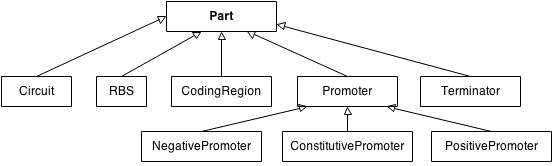
\includegraphics{part_uml.png}
\caption{Hierarchy of AOSB built in Part classes.}\end{figure}

All Parts have the capacity to be connected to a Molecule class. Of the standard parts, \code{CodingRegion}, \code{PositivePromoter} and \code{Negative Promoter} require a Molecule class to be specified. For example, in the {\hyperref[tutorial:hello-world]{Hello World}} example, the coding region is initialized with \emph{Protein}, a built in sub class of \emph{Molecule}.

Additionally, the Weaver assigns Part attributes \code{before} and \code{after}, to refer to the Parts before and
after it in the Part list, and a \code{namespace} attribute, referring to the Circuit or Aspect which added it.

\begin{notice}{warning}{Warning:}
Molecules are always used as \textbf{classes}, not as objects. This is because they
represent an interaction of a Part with a \textbf{type} of Molecule, not just a specific
Molecule.

On the other hand, Parts are always used as objects. However, for syntactic
convenience, if a Part requires no parameters to be initialized, \code{addPart()}
accepts Part classes and automatically converts them into objects. This can be seen
in the {\hyperref[tutorial:hello-world]{Hello World}} example: The Promoter, RBS and Terminator Parts are added
as classes. This is equivalent to adding them as an object, i.e.
\code{addPart(Promoter())}. The \code{CodingRegion} class however needs a Molecule to be
instantiated, and thus needs to be added as an object.
\end{notice}

Parts are a central element of AOSB, because they represent the basic building blocks of
the synthetic biology target.

Because each part is a class, new or more concrete Parts and Molecules
can be added in the normal Python way, potentially defining additional attributes:

\begin{Verbatim}[commandchars=\\\{\}]
\PYG{c}{\PYGZsh{} Parts Registry RBS (http://parts.igem.org/Help:Ribosome\PYGZus{}Binding\PYGZus{}Site)}
\PYG{k}{class} \PYG{n+nc}{BBa\PYGZus{}B0030}     \PYG{p}{(}\PYG{n}{RBS}\PYG{p}{)}\PYG{p}{:}
    \PYG{n}{sequence} \PYG{o}{=} \PYG{l+s}{"}\PYG{l+s}{attaaagaggagaaa}\PYG{l+s}{"}
    \PYG{n}{bindingEfficiency} \PYG{o}{=} \PYG{l+m+mf}{0.6}

\PYG{c}{\PYGZsh{} declare that a class of Proteins called exists that are used as markers}
\PYG{k}{class} \PYG{n+nc}{ReporterProtein} \PYG{p}{(}\PYG{n}{Protein}\PYG{p}{)}\PYG{p}{:}
    \PYG{k}{pass}
\end{Verbatim}

Creating new, specialized Parts and Molecules will be a frequent occurance in an
AOSB program,
so the language also provides the \code{declareNewPart} and \code{declareNewMolecule}
convenience functions:

\begin{Verbatim}[commandchars=\\\{\}]
\PYG{n}{declareNewMolecule}\PYG{p}{(}\PYG{l+s}{"}\PYG{l+s}{GFP}\PYG{l+s}{"}\PYG{p}{,}\PYG{n}{ReporterProtein}\PYG{p}{)}
\PYG{c}{\PYGZsh{} after this line, a new class GFP has been exported to the namespace}

\PYG{n}{declareNewPart}\PYG{p}{(}\PYG{l+s}{"}\PYG{l+s}{GFPCodingRegion}\PYG{l+s}{"}\PYG{p}{,}\PYG{n}{CodingRegion}\PYG{p}{,}\PYG{n}{GFP}\PYG{p}{)}
\PYG{c}{\PYGZsh{} a new class GFPCodingRegion, subtype of CodingRegion has been created}
\PYG{c}{\PYGZsh{} the third parameter can specify a Molecule}
\end{Verbatim}

\code{declareNewMolecule} can accept more than one parent class of type Molecule, so that
a Molecule could be tagged by various classes, e.g. ReporterProtein, FluorescentProtein,
etc. This will be useful once we start selecting Molecules with point cuts. See the
reference on {\hyperref[modules/index:aosb.core.declareNewPart]{\code{declareNewPart()}}} and
{\hyperref[modules/index:aosb.core.declareNewMolecule]{\code{declareNewMolecule()}}} for more information.


\section{Aspects}
\label{tutorial:aspects}
The purpose of AOSB is to allow synthetic biology core and cross-cutting concerns
to be modularized. This requires constructs that define weaving rules, which can be
used to manipulate the execution flow, i.e. the genetic circuit.

Weaving rules are bundled into ``Aspect classes'':

\begin{Verbatim}[commandchars=\\\{\}]
\PYG{k}{class} \PYG{n+nc}{EmptyAspect}\PYG{p}{(}\PYG{n}{Aspect}\PYG{p}{)}\PYG{p}{:}
    \PYG{k}{def} \PYG{n+nf}{mainAspect}\PYG{p}{(}\PYG{n+nb+bp}{self}\PYG{p}{)}\PYG{p}{:}
        \PYG{c}{\PYGZsh{} advice must be registered here}
        \PYG{k}{pass}
\end{Verbatim}


\subsection{Design Rules Example}
\label{tutorial:design-rules-example}
A simple example shows how an Aspect can be used to automatically weave RBS and
Terminator parts around Coding Regions:
\begin{quote}

\begin{Verbatim}[commandchars=\\\{\}]
\PYG{k+kn}{from} \PYG{n+nn}{aosb} \PYG{k+kn}{import} \PYG{o}{*}

\PYG{k}{class} \PYG{n+nc}{CodingGFP}\PYG{p}{(}\PYG{n}{Circuit}\PYG{p}{)}\PYG{p}{:}
    \PYG{k}{def} \PYG{n+nf}{mainCircuit}\PYG{p}{(}\PYG{n+nb+bp}{self}\PYG{p}{)}\PYG{p}{:}
        \PYG{n}{declareNewMolecule}\PYG{p}{(}\PYG{l+s}{'}\PYG{l+s}{GFP}\PYG{l+s}{'}\PYG{p}{)} 
        \PYG{n+nb+bp}{self}\PYG{o}{.}\PYG{n}{addPart}\PYG{p}{(}\PYG{n}{Promoter}\PYG{p}{)}
        \PYG{n+nb+bp}{self}\PYG{o}{.}\PYG{n}{addPart}\PYG{p}{(}\PYG{n}{CodingRegion}\PYG{p}{(}\PYG{n}{GFP}\PYG{p}{)}\PYG{p}{)}
        
\PYG{k}{class} \PYG{n+nc}{DesignRules}\PYG{p}{(}\PYG{n}{Aspect}\PYG{p}{)}\PYG{p}{:}
    \PYG{k}{def} \PYG{n+nf}{mainAspect}\PYG{p}{(}\PYG{n+nb+bp}{self}\PYG{p}{)}\PYG{p}{:}
        \PYG{n}{anyCodingRegion} \PYG{o}{=} \PYG{n}{PartSignature}\PYG{p}{(}\PYG{l+s}{'}\PYG{l+s}{*.CodingRegion+}\PYG{l+s}{'}\PYG{p}{)}
        
        \PYG{n}{beforeCodingRegion} \PYG{o}{=} \PYG{n}{PointCut}\PYG{p}{(}\PYG{n}{anyCodingRegion}\PYG{p}{,}\PYG{n}{PointCut}\PYG{o}{.}\PYG{n}{BEFORE}\PYG{p}{)}
        \PYG{n}{afterCodingRegion} \PYG{o}{=} \PYG{n}{PointCut}\PYG{p}{(}\PYG{n}{anyCodingRegion}\PYG{p}{,}\PYG{n}{PointCut}\PYG{o}{.}\PYG{n}{AFTER}\PYG{p}{)}
        
        \PYG{n+nb+bp}{self}\PYG{o}{.}\PYG{n}{addAdvice}\PYG{p}{(}\PYG{n}{beforeCodingRegion}\PYG{p}{,}\PYG{n+nb+bp}{self}\PYG{o}{.}\PYG{n}{insertRBS}\PYG{p}{)}
        \PYG{n+nb+bp}{self}\PYG{o}{.}\PYG{n}{addAdvice}\PYG{p}{(}\PYG{n}{afterCodingRegion}\PYG{p}{,}\PYG{n+nb+bp}{self}\PYG{o}{.}\PYG{n}{insertTerminator}\PYG{p}{)}
    
    \PYG{k}{def} \PYG{n+nf}{insertRBS}\PYG{p}{(}\PYG{n+nb+bp}{self}\PYG{p}{,}\PYG{n}{context}\PYG{p}{)}\PYG{p}{:}
        \PYG{n+nb+bp}{self}\PYG{o}{.}\PYG{n}{addPart}\PYG{p}{(}\PYG{n}{RBS}\PYG{p}{)}
    
    \PYG{k}{def} \PYG{n+nf}{insertTerminator}\PYG{p}{(}\PYG{n+nb+bp}{self}\PYG{p}{,}\PYG{n}{context}\PYG{p}{)}\PYG{p}{:}
        \PYG{n+nb+bp}{self}\PYG{o}{.}\PYG{n}{addPart}\PYG{p}{(}\PYG{n}{Terminator}\PYG{p}{)}

\PYG{n}{compiledDesign} \PYG{o}{=} \PYG{n}{Weaver}\PYG{p}{(}\PYG{n}{CodingGFP}\PYG{p}{,}\PYG{n}{DesignRules}\PYG{p}{)}\PYG{o}{.}\PYG{n}{output}\PYG{p}{(}\PYG{p}{)}
\PYG{k}{print} \PYG{n}{compiledDesign}
\end{Verbatim}
\end{quote}

The output of this program is:

\begin{Verbatim}[commandchars=\\\{\}]
\PYG{n}{Promoter}\PYG{o}{+}\PYG{n}{RBS}\PYG{o}{+}\PYG{n}{CodingRegion}\PYG{p}{(}\PYG{n}{codesFor} \PYG{o}{=} \PYG{n}{GFP}\PYG{p}{)}\PYG{o}{+}\PYG{n}{Terminator}
\end{Verbatim}

In the following sections, the constructs introduced in the example will be covered
in detail.

The simple defines the ``core concern'', GFP coded under an unspecified Promoter,
in the CodingGFP Circuit \emph{(lines 3-7)}. The DesignRules Aspect \emph{(lines 9-23)} defines
two advice methods, \code{insertRBS'' and {}`{}`insertTerinator}. Each Aspect has to implement
a \code{mainAspect()} method, similarly to a Circuit's \code{mainCircuit()}. During the
execution of \code{mainAspect()}, all advice of the Aspect must be declared. In the example
\emph{(lines 16 and 17)}, the two advice methods are attached two the appropriate PointCut and
declared using {\hyperref[modules/index:aosb.core.Aspect.addAdvice]{\code{addAdvice()}}}.

Lastly, CodingGFP and DesignRules are given as inputs to the Weaver \emph{(lines 25)}.

The Weaver now first constructs the classes and creates a list of all advice, by calling
DesignRule's \code{mainAspect()}. Then, it calls CodingGFP's \code{mainCircuit()} method.
When the CodingRegion is added \emph{(line 7)}, the Weaver is able to match the advice from
DesignRules and inserts a call to \code{insertRBS()} before adding the CodingRegion, and a
call to \code{insertTerminator()} after it.


\section{Point Cuts}
\label{tutorial:point-cuts}
A \code{PointCut} matches specific join points in the genetic circuit execution flow.

The \code{Point Cut constructor} requires a
PartSignature and an operator of type \code{PointCut.BEFORE} / \code{AFTER} or \code{REPLACE},
which specifies how the matching join point should be manipulated.


\subsection{Simple Part Signatures}
\label{tutorial:simple-part-signatures}
In the {\hyperref[tutorial:design-rules-example]{Design Rules Example}} we have seen an example of a simple PartSignature:

\begin{Verbatim}[commandchars=\\\{\}]
.. code-block:: python
\end{Verbatim}
\begin{quote}

PartSignature(`{\color{red}\bfseries{}*}.CodingRegion+')
\end{quote}

This part matches any part of type (or sub-type) \code{CodingRegion}.

A Part Signature consists of three parts. Firstly, it can specify a namespace of a Part,
i.e. the Circuit or Aspect which has added it. Secondly, it can specify the part itself.
Thirdly, it can optionally specify a Molecule the part should be connected to. Matching
is done on the name of the type.

\begin{Verbatim}[commandchars=\\\{\}]
\PYG{n}{NameSpaceTypeName}\PYG{o}{.}\PYG{n}{PartTypeName}\PYG{p}{(}\PYG{n}{MoleculeName}\PYG{p}{)}
\end{Verbatim}

Additionally, the wild card operator \code{*} will match any name, and the \code{+} will make
any type or subtype a match. Furthermore, a \code{!} at the beginning of any element of the
signature will invert it.

\textbf{Examples}

\begin{Verbatim}[commandchars=\\\{\}]
\PYG{l+s}{"}\PYG{l+s}{Circuit+.BB*(*)}\PYG{l+s}{"}
\end{Verbatim}

will match any part, which has been added by a Circuit (i.e. not by an Aspect) and whose
type name begins with ``BB'' (e.g. by naming convention, a BioBrick part). The molecule
connection is irrelevant, so \code{(*)} for the molecule element of the signature is
equivalent to leavning it out.

\begin{Verbatim}[commandchars=\\\{\}]
\PYG{l+s}{"}\PYG{l+s}{Aspect+.Promoter+(TranscriptionFactor+)}\PYG{l+s}{"}
\end{Verbatim}

will match any Promoter (including subtypes such as NegativePromoter, PositivePromoter,
any any user-defined types) that has been added by an Aspect and is regulated by a
TranscriptionFactor.

\begin{Verbatim}[commandchars=\\\{\}]
\PYG{l+s}{"}\PYG{l+s}{!SimpleAspect.*(!GFP)}\PYG{l+s}{"}
\end{Verbatim}

will match any Part not being connected to GFP which has not been added by an Aspect
called SimpleAspect.

Thus, by constructing a sensible typing hierarchy of Parts and Molecules and by
establishing a rigorous naming convention, Point Cuts are able to select groups of
Parts based on precise features.


\subsection{Point Cut Expressions}
\label{tutorial:point-cut-expressions}
Additionally, Part Signatures can be connected into expressions, using the \code{\&}, \code{\textbar{}}
and \code{\%} operators, which stand for boolean-and, boolean-or and concatenation,
respectively.

\textbf{Examples}

\begin{Verbatim}[commandchars=\\\{\}]
\PYG{n}{PartSelector}\PYG{p}{(}\PYG{l+s}{'}\PYG{l+s}{*.NegativePromoter+}\PYG{l+s}{'}\PYG{p}{)} \PYG{o}{\textbar{}} \PYG{n}{PartSelector}\PYG{p}{(}\PYG{l+s}{'}\PYG{l+s}{*.PositivePromoter+}\PYG{l+s}{'}\PYG{p}{)}
\end{Verbatim}

will match any part whose (sub)type is either \code{NegativePromoter} or \code{PositivePromoter}.

\begin{Verbatim}[commandchars=\\\{\}]
\PYG{n}{PartSelector}\PYG{p}{(}\PYG{l+s}{'}\PYG{l+s}{*.*(TranscriptionFactor+)}\PYG{l+s}{'}\PYG{p}{)} \PYG{o}{\&} \PYG{n}{PartSelector}\PYG{p}{(}\PYG{l+s}{'}\PYG{l+s}{*.*(ReporterProtein+))}
\end{Verbatim}

will match any part whose molecule is both a TranscriptionFactor and a ReporterProtein.

\begin{Verbatim}[commandchars=\\\{\}]
\PYG{n}{PartSelector}\PYG{p}{(}\PYG{l+s}{'}\PYG{l+s}{*.RBS+}\PYG{l+s}{'}\PYG{p}{)} \PYG{o}{\PYGZpc{}} \PYG{n}{PartSelector}\PYG{p}{(}\PYG{l+s}{'}\PYG{l+s}{*.CodingRegion+}\PYG{l+s}{'}\PYG{p}{)}
\end{Verbatim}

will match any CodingRegion, which has an RBS part immediately before it.

Using these operators, complex Point Cut expressions can be built.
All operators are left-associative, so there is no clear precedence between operators.
Rather, precedence should be explicitly defined using parentheses.

Additionally, parts of a formula can be inverted using a \code{PointCutExpressionNot()} node,
which does not have an overloaded Python operator:

\begin{Verbatim}[commandchars=\\\{\}]
\PYG{n}{PointCutExpressionNot}\PYG{p}{(}\PYG{l+s}{'}\PYG{l+s}{*.Terminator+}\PYG{l+s}{'}\PYG{p}{)}
\end{Verbatim}

will match any Part not matched by \code{'*.Terminator+'}


\section{Advice}
\label{tutorial:advice}
Advice is the code woven into the execution flow.  An \code{Advice} consists of a PointCut,
to select the location of where the code should be inserted, and a method of the Aspect.

An advice method belongs to the Aspect, and can access and store attributes via the \code{self} parameter. An advice method must also accept a second Parameter called \code{context}:

\begin{Verbatim}[commandchars=\\\{\}]
\PYG{k}{def} \PYG{n+nf}{adviceMethod}\PYG{p}{(}\PYG{n+nb+bp}{self}\PYG{p}{,}\PYG{n}{context}\PYG{p}{)}\PYG{p}{:}
    \PYG{c}{\PYGZsh{} self.addPart() could be used here}
    \PYG{k}{pass}
\end{Verbatim}

\code{context} is of type {\hyperref[modules/index:aosb.core.PointCutContext]{\code{PointCutContext}}}, which has
a \code{PointCutContext.part} attribute, referencing the part that was matched by the
PointCut of the advice.

Additionally, \code{context} has an {\hyperref[modules/index:aosb.core.PointCutContext.isWithin]{\code{isWithin()}}} method, which
can be used to search for Circuits or Aspects on the advice call stack. For example, this can be used to
make sure that an advice is not recursively executing on itself.


\subsection{Example: Print Advice Stack}
\label{tutorial:example-print-advice-stack}
Based on the previous {\hyperref[tutorial:design-rules-example]{Design Rules Example}} we can quickly add an aspect to print a stack trace:

\begin{Verbatim}[commandchars=\\\{\}]
\PYG{k+kn}{from} \PYG{n+nn}{aosb} \PYG{k+kn}{import} \PYG{o}{*}

\PYG{k}{class} \PYG{n+nc}{CodingGFP}\PYG{p}{(}\PYG{n}{Circuit}\PYG{p}{)}\PYG{p}{:}
    \PYG{k}{def} \PYG{n+nf}{mainCircuit}\PYG{p}{(}\PYG{n+nb+bp}{self}\PYG{p}{)}\PYG{p}{:}
        \PYG{n}{declareNewMolecule}\PYG{p}{(}\PYG{l+s}{'}\PYG{l+s}{GFP}\PYG{l+s}{'}\PYG{p}{)} 
        \PYG{n+nb+bp}{self}\PYG{o}{.}\PYG{n}{addPart}\PYG{p}{(}\PYG{n}{Promoter}\PYG{p}{)}
        \PYG{n+nb+bp}{self}\PYG{o}{.}\PYG{n}{addPart}\PYG{p}{(}\PYG{n}{CodingRegion}\PYG{p}{(}\PYG{n}{GFP}\PYG{p}{)}\PYG{p}{)}
        
\PYG{k}{class} \PYG{n+nc}{DesignRules}\PYG{p}{(}\PYG{n}{Aspect}\PYG{p}{)}\PYG{p}{:}
    \PYG{k}{def} \PYG{n+nf}{mainAspect}\PYG{p}{(}\PYG{n+nb+bp}{self}\PYG{p}{)}\PYG{p}{:}
        \PYG{n}{anyCodingRegion} \PYG{o}{=} \PYG{n}{PartSignature}\PYG{p}{(}\PYG{l+s}{'}\PYG{l+s}{*.CodingRegion+}\PYG{l+s}{'}\PYG{p}{)}
        
        \PYG{n}{beforeCodingRegion} \PYG{o}{=} \PYG{n}{PointCut}\PYG{p}{(}\PYG{n}{anyCodingRegion}\PYG{p}{,}\PYG{n}{PointCut}\PYG{o}{.}\PYG{n}{BEFORE}\PYG{p}{)}
        \PYG{n}{afterCodingRegion} \PYG{o}{=} \PYG{n}{PointCut}\PYG{p}{(}\PYG{n}{anyCodingRegion}\PYG{p}{,}\PYG{n}{PointCut}\PYG{o}{.}\PYG{n}{AFTER}\PYG{p}{)}
        
        \PYG{n+nb+bp}{self}\PYG{o}{.}\PYG{n}{addAdvice}\PYG{p}{(}\PYG{n}{beforeCodingRegion}\PYG{p}{,}\PYG{n+nb+bp}{self}\PYG{o}{.}\PYG{n}{insertRBS}\PYG{p}{)}
        \PYG{n+nb+bp}{self}\PYG{o}{.}\PYG{n}{addAdvice}\PYG{p}{(}\PYG{n}{afterCodingRegion}\PYG{p}{,}\PYG{n+nb+bp}{self}\PYG{o}{.}\PYG{n}{insertTerminator}\PYG{p}{)}
    
    \PYG{k}{def} \PYG{n+nf}{insertRBS}\PYG{p}{(}\PYG{n+nb+bp}{self}\PYG{p}{,}\PYG{n}{context}\PYG{p}{)}\PYG{p}{:}
        \PYG{n+nb+bp}{self}\PYG{o}{.}\PYG{n}{addPart}\PYG{p}{(}\PYG{n}{RBS}\PYG{p}{)}
    
    \PYG{k}{def} \PYG{n+nf}{insertTerminator}\PYG{p}{(}\PYG{n+nb+bp}{self}\PYG{p}{,}\PYG{n}{context}\PYG{p}{)}\PYG{p}{:}
        \PYG{n+nb+bp}{self}\PYG{o}{.}\PYG{n}{addPart}\PYG{p}{(}\PYG{n}{Terminator}\PYG{p}{)}
        
\PYG{k}{class} \PYG{n+nc}{PrintStack}\PYG{p}{(}\PYG{n}{Aspect}\PYG{p}{)}\PYG{p}{:}
    \PYG{k}{def} \PYG{n+nf}{mainAspect}\PYG{p}{(}\PYG{n+nb+bp}{self}\PYG{p}{)}\PYG{p}{:}
        \PYG{n+nb+bp}{self}\PYG{o}{.}\PYG{n}{addAdvice}\PYG{p}{(}\PYG{n}{PointCut}\PYG{p}{(}\PYG{l+s}{'}\PYG{l+s}{*.*}\PYG{l+s}{'}\PYG{p}{,}\PYG{n}{PointCut}\PYG{o}{.}\PYG{n}{AFTER}\PYG{p}{)}\PYG{p}{,}\PYG{n+nb+bp}{self}\PYG{o}{.}\PYG{n}{printStack}\PYG{p}{)}
    
    \PYG{k}{def} \PYG{n+nf}{printStack}\PYG{p}{(}\PYG{n+nb+bp}{self}\PYG{p}{,}\PYG{n}{context}\PYG{p}{)}\PYG{p}{:}
        \PYG{k}{print} \PYG{l+s}{'}\PYG{l+s}{,}\PYG{l+s}{'}\PYG{o}{.}\PYG{n}{join}\PYG{p}{(}\PYG{n+nb}{str}\PYG{p}{(}\PYG{n}{context}\PYG{o}{.}\PYG{n}{within}\PYG{p}{[}\PYG{n}{i}\PYG{p}{]}\PYG{p}{)} \PYG{k}{for} \PYG{n}{i} \PYG{o+ow}{in} \PYG{n+nb}{range}\PYG{p}{(}\PYG{n+nb}{len}\PYG{p}{(}\PYG{n}{context}\PYG{o}{.}\PYG{n}{within}\PYG{p}{)}\PYG{p}{)}\PYG{p}{)} \PYG{o}{+} \PYG{l+s}{"}\PYG{l+s}{ add: }\PYG{l+s}{"} \PYG{o}{+} \PYG{n+nb}{str}\PYG{p}{(}\PYG{n}{context}\PYG{o}{.}\PYG{n}{part}\PYG{p}{)}
    

\PYG{n}{compiledDesign} \PYG{o}{=} \PYG{n}{Weaver}\PYG{p}{(}\PYG{n}{CodingGFP}\PYG{p}{,}\PYG{n}{DesignRules}\PYG{p}{,}\PYG{n}{PrintStack}\PYG{p}{)}\PYG{o}{.}\PYG{n}{output}\PYG{p}{(}\PYG{p}{)}
\PYG{k}{print} \PYG{n}{compiledDesign}
\end{Verbatim}

This will give the following output:

\begin{Verbatim}[commandchars=\\\{\}]
CodingGFP add: Promoter
CodingGFP,\textless{}\_\_main\_\_.DesignRules object at 0x7f8f42987a50\textgreater{} add: RBS
CodingGFP,\textless{}\_\_main\_\_.DesignRules object at 0x7f8f42987a50\textgreater{} add: Terminator
CodingGFP add: CodingRegion(codesFor = GFP)
Promoter+RBS+CodingRegion(codesFor = GFP)+Terminator
\end{Verbatim}

\code{CodingGFP} has a nicer string representation, which it inherits from Part (see Composites).


\subsection{before and after Point Cuts}
\label{tutorial:before-and-after-point-cuts}
We have already encountered the simpler Before and After Point Cuts. They inject the advice code
immediately before or after the join point selected by the Point Cut, as would be expected.
\begin{figure}[htbp]
\centering
\capstart

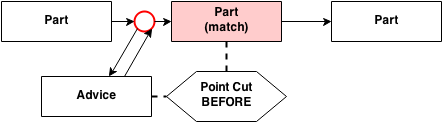
\includegraphics{point_cut_before.png}
\caption{Advice weaving at a join point selected by a BEFORE Point Cut}\end{figure}
\begin{figure}[htbp]
\centering
\capstart

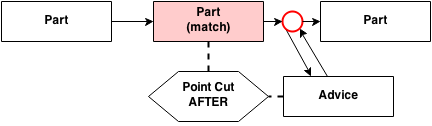
\includegraphics{point_cut_after.png}
\caption{Advice weaving at a join point selected by an AFTER Point Cut}\end{figure}


\subsection{replace Point Cuts}
\label{tutorial:replace-point-cuts}\begin{figure}[htbp]
\centering
\capstart

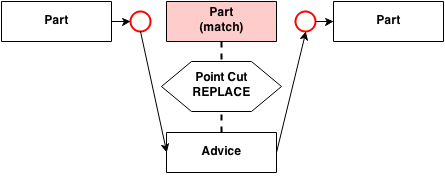
\includegraphics{point_cut_replace.png}
\caption{Advice on a replace Point Cut is executed instead of the Part.}\end{figure}


\subsection{Precedence}
\label{tutorial:precedence}
What if more than one Point Cut matches a given Join Point? Unless a precedence is explicitly
set, the behavior is undefined.

\code{addAdvice()} takes an optional third parameter - an integer between \code{Advice.MINPRECEDENCE} \emph{(0)}
and \code{Advice.MAXPRECEDENCE} \emph{(100)}

Advice which are added without specifying a precedence, are given minimal precedence by default. Higher precedence Advice is are deemed more important than those of low precedence.

For two Advice sharing a BEFORE Point Cut, this means that the high precedence advice will execute \textbf{before} the low precedence one. If both advice have the same precedence, their order is undefined.

For two Advice sharing an AFTER Point Cut, the high precedence advice will execute \textbf{after} the low precedence one. If both advice have the same precedence, their order is undefined.

For two Advice sharing a REPLACEMENT Point Cut, the high precedence advice will execute, whereas any lower precedence advice will be ignored.

If many Point Cuts match a Join Point, first the before advice will execute starting from the highest precedence. After the last before advice, the part will be added. Then the lowest precedence after advice will execute until the highest after advice. If a replacement advice occurs at some point, any lower before or after advice will be ignored. However, all after advice of similar or higher precedence will still execute.
\begin{figure}[htbp]
\centering
\capstart

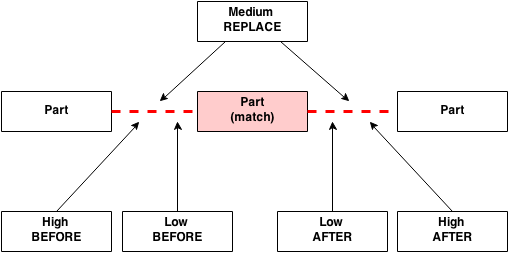
\includegraphics{point_cut_precedence.png}
\caption{In this example, the low advice and the matched Part will not be executed, as they have been replaced
by the medium Advice}\end{figure}


\section{Type Advice}
\label{tutorial:type-advice}
Apart from normal Advice, which changes the execution flow, it is also possible to modify the Molecule
and Part types using type advice. For example, one Aspect could add sequence information to a whole range
of Parts; another could add modelling rules to Parts based on features selected by a \code{PartSignature}.

Analogously to \code{addAdvice()}, type advice can be added with


\subsection{Adding type advice to Parts}
\label{tutorial:adding-type-advice-to-parts}
Analogously to adding new Advice with \code{addAdvice()}, Type Advice can be
added via {\hyperref[modules/index:aosb.core.Aspect.addTypeAdvice]{\code{addTypeAdvice()}}}:

\begin{Verbatim}[commandchars=\\\{\}]
\PYG{k}{def} \PYG{n+nf}{mainAspect}\PYG{p}{(}\PYG{n+nb+bp}{self}\PYG{p}{)}\PYG{p}{:}
    \PYG{n+nb+bp}{self}\PYG{o}{.}\PYG{n}{addTypeAdvice}\PYG{p}{(}\PYG{n}{PartSignature}\PYG{p}{(}\PYG{l+s}{'}\PYG{l+s}{*.*}\PYG{l+s}{'}\PYG{p}{)}\PYG{p}{,}\PYG{n+nb+bp}{True}\PYG{p}{,}\PYG{l+s}{"}\PYG{l+s}{isPart}\PYG{l+s}{"}\PYG{p}{)}
\end{Verbatim}

\code{addTypeAdvice} requires three parameters: A \code{PartSignature} to select the Part, an
attribute to add to the Part type, and a name under which this Part should appear.

If the attribute is a method, it is given two parameters: \code{self}, referring to the
Aspect, and \code{part}, referring to the Part object:

\begin{Verbatim}[commandchars=\\\{\}]
class AnAspect(Aspect):
    def mainAspect(self):
        self.addTypeAdvice(PartSignature('*.*'),self.typeAdviceMethod,"sayHello")

    def typeAdviceMethod(self,part)
        print "Hello from "+str(part)
\end{Verbatim}

Type Advice can also be added to \code{Molecules} using the same \code{addTypeAdvice()} method.
This requires changing the first parameter to a {\hyperref[modules/index:aosb.core.MoleculeSignature]{\code{MoleculeSignature}}}:

\begin{Verbatim}[commandchars=\\\{\}]
\PYG{k}{def} \PYG{n+nf}{mainAspect}\PYG{p}{(}\PYG{n+nb+bp}{self}\PYG{p}{)}\PYG{p}{:}
    \PYG{n+nb+bp}{self}\PYG{o}{.}\PYG{n}{addTypeAdvice}\PYG{p}{(}\PYG{n}{MoleculeSignature}\PYG{p}{(}\PYG{l+s}{'}\PYG{l+s}{TranscriptionFactor+}\PYG{l+s}{'}\PYG{p}{)}\PYG{p}{,}\PYG{n+nb+bp}{True}\PYG{p}{,}\PYG{l+s}{"}\PYG{l+s}{isTranscriptionFactor}\PYG{l+s}{"}\PYG{p}{)}
\end{Verbatim}

The \code{MoleculeSignature} is simply the element of the PartSignature within the parantheses.


\subsection{Type Advice Example}
\label{tutorial:type-advice-example}
Here is a simple example to add a method to Promoter types to print if they are regulated or not.

\begin{Verbatim}[commandchars=\\\{\}]
\PYG{k+kn}{from} \PYG{n+nn}{aosb} \PYG{k+kn}{import} \PYG{o}{*}

\PYG{k}{class} \PYG{n+nc}{TwoPromoters}\PYG{p}{(}\PYG{n}{Circuit}\PYG{p}{)}\PYG{p}{:}
    \PYG{k}{def} \PYG{n+nf}{mainCircuit}\PYG{p}{(}\PYG{n+nb+bp}{self}\PYG{p}{)}\PYG{p}{:}
        \PYG{n+nb+bp}{self}\PYG{o}{.}\PYG{n}{addPart}\PYG{p}{(}\PYG{n}{Promoter}\PYG{p}{)}
        \PYG{n+nb+bp}{self}\PYG{o}{.}\PYG{n}{addPart}\PYG{p}{(}\PYG{n}{NegativePromoter}\PYG{p}{(}\PYG{n}{Protein}\PYG{p}{)}\PYG{p}{)}
        
\PYG{k}{class} \PYG{n+nc}{PromoterTypeAdvice}\PYG{p}{(}\PYG{n}{Aspect}\PYG{p}{)}\PYG{p}{:}
    \PYG{k}{def} \PYG{n+nf}{mainAspect}\PYG{p}{(}\PYG{n+nb+bp}{self}\PYG{p}{)}\PYG{p}{:}
        \PYG{c}{\PYGZsh{} define three signatures}
        \PYG{n}{nonRegulatedPromoterSignature} \PYG{o}{=} \PYG{n}{PartSignature}\PYG{p}{(}\PYG{l+s}{'}\PYG{l+s}{*.Promoter+()}\PYG{l+s}{'}\PYG{p}{)}
        \PYG{n}{regulatedPromoterSignature} \PYG{o}{=} \PYG{n}{PartSignature}\PYG{p}{(}\PYG{l+s}{'}\PYG{l+s}{*.Promoter+(Molecule+)}\PYG{l+s}{'}\PYG{p}{)}
        \PYG{n}{anyPromoterSignature} \PYG{o}{=} \PYG{n}{PartSignature}\PYG{p}{(}\PYG{l+s}{'}\PYG{l+s}{*.Promoter+}\PYG{l+s}{'}\PYG{p}{)}
        
        \PYG{c}{\PYGZsh{} add Boolean Attribute "isRegulated" to two different types of Promoters}
        \PYG{n+nb+bp}{self}\PYG{o}{.}\PYG{n}{addTypeAdvice}\PYG{p}{(}\PYG{n}{nonRegulatedPromoterSignature}\PYG{p}{,}\PYG{n+nb+bp}{False}\PYG{p}{,}\PYG{l+s}{"}\PYG{l+s}{isRegulated}\PYG{l+s}{"}\PYG{p}{)}
        \PYG{n+nb+bp}{self}\PYG{o}{.}\PYG{n}{addTypeAdvice}\PYG{p}{(}\PYG{n}{regulatedPromoterSignature}\PYG{p}{,}\PYG{n+nb+bp}{True}\PYG{p}{,}\PYG{l+s}{"}\PYG{l+s}{isRegulated}\PYG{l+s}{"}\PYG{p}{)}
        
        \PYG{c}{\PYGZsh{} add a type advice method}
        \PYG{n+nb+bp}{self}\PYG{o}{.}\PYG{n}{addTypeAdvice}\PYG{p}{(}\PYG{n}{anyPromoterSignature}\PYG{p}{,}\PYG{n+nb+bp}{self}\PYG{o}{.}\PYG{n}{printIsRegulated}\PYG{p}{,}\PYG{l+s}{"}\PYG{l+s}{printIsRegulated}\PYG{l+s}{"}\PYG{p}{)}
        
    \PYG{k}{def} \PYG{n+nf}{printIsRegulated}\PYG{p}{(}\PYG{n+nb+bp}{self}\PYG{p}{,}\PYG{n}{part}\PYG{p}{)}\PYG{p}{:}
        \PYG{k}{if} \PYG{n}{part}\PYG{o}{.}\PYG{n}{isRegulated} \PYG{o}{==} \PYG{n+nb+bp}{False}\PYG{p}{:}
            \PYG{k}{print} \PYG{n+nb}{str}\PYG{p}{(}\PYG{n}{part}\PYG{p}{)}\PYG{o}{+}\PYG{l+s}{"}\PYG{l+s}{ is not regulated by a Molecule.}\PYG{l+s}{"}
        \PYG{k}{else}\PYG{p}{:}
            \PYG{k}{print} \PYG{n+nb}{str}\PYG{p}{(}\PYG{n}{part}\PYG{p}{)}\PYG{o}{+}\PYG{l+s}{"}\PYG{l+s}{ is regulated by a Molecule.}\PYG{l+s}{"}

\PYG{n}{compiledDesign} \PYG{o}{=} \PYG{n}{Weaver}\PYG{p}{(}\PYG{n}{TwoPromoters}\PYG{p}{,}\PYG{n}{PromoterTypeAdvice}\PYG{p}{)}\PYG{o}{.}\PYG{n}{output}\PYG{p}{(}\PYG{p}{)}
\PYG{k}{for} \PYG{n}{part} \PYG{o+ow}{in} \PYG{n}{compiledDesign}\PYG{o}{.}\PYG{n}{partList}\PYG{p}{:}
    \PYG{n}{part}\PYG{o}{.}\PYG{n}{printIsRegulated}\PYG{p}{(}\PYG{p}{)}
\end{Verbatim}

The output will be:

\begin{Verbatim}[commandchars=\\\{\}]
Promoter is not regulated by a Molecule.
NegativePromoter(regulatedBy = Protein) is regulated by a Molecule.
\end{Verbatim}


\section{Weaver Output Advice}
\label{tutorial:weaver-output-advice}
The last item to cover is the {\hyperref[modules/index:aosb.core.Weaver.WeaverOutput]{\code{WeaverOutput}}} class, a
container object holding the results of the Weaver compilation and returned by \code{Weaver.output()}:

\begin{Verbatim}[commandchars=\\\{\}]
\PYG{n}{compiledDesign} \PYG{o}{=} \PYG{n}{Weaver}\PYG{p}{(}\PYG{n}{ACircuit}\PYG{p}{,}\PYG{n}{AnAspect}\PYG{p}{,}\PYG{n}{AnotherAspect}\PYG{p}{)}\PYG{o}{.}\PYG{n}{output}\PYG{p}{(}\PYG{p}{)}
\end{Verbatim}

By default, \code{WeaverOutput} has two attributes. \code{partList}, holding the list of the parts in order of execution,
and \code{moleculeList} a list of all types of Molecules used in the system. The class also overloads \code{\_\_str\_\_} to provide
a nice string output of the compiles design, which we have used in previous examples.

An Aspect can also declare output advice to the \code{WeaverOutput}. For example, this allows an Aspect implementing a rule-based modelling
concern to define additional \code{WeaverOutput} methods, such as \code{printModel()}.

The mechanism is very similar to Type Advice:

\begin{Verbatim}[commandchars=\\\{\}]
\PYG{k}{def} \PYG{n+nf}{mainAspect}\PYG{p}{(}\PYG{n+nb+bp}{self}\PYG{p}{)}\PYG{p}{:}
    \PYG{n}{addWeaverOutput}\PYG{p}{(}\PYG{n+nb+bp}{self}\PYG{o}{.}\PYG{n}{newOutputMethod}\PYG{p}{)}

\PYG{k}{def} \PYG{n+nf}{newOutputMethod}\PYG{p}{(}\PYG{n+nb+bp}{self}\PYG{p}{,}\PYG{n}{weaverOutput}\PYG{p}{)}\PYG{p}{:}
    \PYG{k}{pass}
\end{Verbatim}

\code{addWeaverOutput()} has only one parameter which must refer to a method of the Aspect. This weaver output advice method must accept
two parameters, \code{self} to refer to the Aspect, and \code{weaverOutput} to refer to the \code{WeaverOutput} object. Unlike
\code{addTypeAdvice()}, \code{addWeaverOutput} requires no name for the new attribute. Instead, the new method for \code{WeaverOutput} will
automatically have the same name.


\subsection{Example: Print number of parts}
\label{tutorial:example-print-number-of-parts}
\begin{Verbatim}[commandchars=\\\{\}]
\PYG{k+kn}{from} \PYG{n+nn}{aosb} \PYG{k+kn}{import} \PYG{o}{*}

\PYG{k}{class} \PYG{n+nc}{CodingGFP}\PYG{p}{(}\PYG{n}{Circuit}\PYG{p}{)}\PYG{p}{:}
    \PYG{k}{def} \PYG{n+nf}{mainCircuit}\PYG{p}{(}\PYG{n+nb+bp}{self}\PYG{p}{)}\PYG{p}{:}
        \PYG{n}{declareNewMolecule}\PYG{p}{(}\PYG{l+s}{'}\PYG{l+s}{GFP}\PYG{l+s}{'}\PYG{p}{)} 
        \PYG{n+nb+bp}{self}\PYG{o}{.}\PYG{n}{addPart}\PYG{p}{(}\PYG{n}{Promoter}\PYG{p}{)}
        \PYG{n+nb+bp}{self}\PYG{o}{.}\PYG{n}{addPart}\PYG{p}{(}\PYG{n}{CodingRegion}\PYG{p}{(}\PYG{n}{GFP}\PYG{p}{)}\PYG{p}{)}
        
\PYG{k}{class} \PYG{n+nc}{DesignRules}\PYG{p}{(}\PYG{n}{Aspect}\PYG{p}{)}\PYG{p}{:}
    \PYG{k}{def} \PYG{n+nf}{mainAspect}\PYG{p}{(}\PYG{n+nb+bp}{self}\PYG{p}{)}\PYG{p}{:}
        \PYG{n}{anyCodingRegion} \PYG{o}{=} \PYG{n}{PartSignature}\PYG{p}{(}\PYG{l+s}{'}\PYG{l+s}{*.CodingRegion+}\PYG{l+s}{'}\PYG{p}{)}
        
        \PYG{n}{beforeCodingRegion} \PYG{o}{=} \PYG{n}{PointCut}\PYG{p}{(}\PYG{n}{anyCodingRegion}\PYG{p}{,}\PYG{n}{PointCut}\PYG{o}{.}\PYG{n}{BEFORE}\PYG{p}{)}
        \PYG{n}{afterCodingRegion} \PYG{o}{=} \PYG{n}{PointCut}\PYG{p}{(}\PYG{n}{anyCodingRegion}\PYG{p}{,}\PYG{n}{PointCut}\PYG{o}{.}\PYG{n}{AFTER}\PYG{p}{)}
        
        \PYG{n+nb+bp}{self}\PYG{o}{.}\PYG{n}{addAdvice}\PYG{p}{(}\PYG{n}{beforeCodingRegion}\PYG{p}{,}\PYG{n+nb+bp}{self}\PYG{o}{.}\PYG{n}{insertRBS}\PYG{p}{)}
        \PYG{n+nb+bp}{self}\PYG{o}{.}\PYG{n}{addAdvice}\PYG{p}{(}\PYG{n}{afterCodingRegion}\PYG{p}{,}\PYG{n+nb+bp}{self}\PYG{o}{.}\PYG{n}{insertTerminator}\PYG{p}{)}
    
    \PYG{k}{def} \PYG{n+nf}{insertRBS}\PYG{p}{(}\PYG{n+nb+bp}{self}\PYG{p}{,}\PYG{n}{context}\PYG{p}{)}\PYG{p}{:}
        \PYG{n+nb+bp}{self}\PYG{o}{.}\PYG{n}{addPart}\PYG{p}{(}\PYG{n}{RBS}\PYG{p}{)}
    
    \PYG{k}{def} \PYG{n+nf}{insertTerminator}\PYG{p}{(}\PYG{n+nb+bp}{self}\PYG{p}{,}\PYG{n}{context}\PYG{p}{)}\PYG{p}{:}
        \PYG{n+nb+bp}{self}\PYG{o}{.}\PYG{n}{addPart}\PYG{p}{(}\PYG{n}{Terminator}\PYG{p}{)}
        
\PYG{k}{class} \PYG{n+nc}{NumberOfPartsAspect}\PYG{p}{(}\PYG{n}{Aspect}\PYG{p}{)}\PYG{p}{:}
    \PYG{k}{def} \PYG{n+nf}{mainAspect}\PYG{p}{(}\PYG{n+nb+bp}{self}\PYG{p}{)}\PYG{p}{:}
        \PYG{n+nb+bp}{self}\PYG{o}{.}\PYG{n}{addWeaverOutput}\PYG{p}{(}\PYG{n+nb+bp}{self}\PYG{o}{.}\PYG{n}{printNumberOfParts}\PYG{p}{)}
        
    \PYG{k}{def} \PYG{n+nf}{printNumberOfParts}\PYG{p}{(}\PYG{n+nb+bp}{self}\PYG{p}{,}\PYG{n}{weaverOutput}\PYG{p}{)}\PYG{p}{:}
        \PYG{k}{print} \PYG{l+s}{"}\PYG{l+s}{The design has }\PYG{l+s}{"}\PYG{o}{+}\PYG{n+nb}{str}\PYG{p}{(}\PYG{n+nb}{len}\PYG{p}{(}\PYG{n}{weaverOutput}\PYG{o}{.}\PYG{n}{partList}\PYG{p}{)}\PYG{p}{)}\PYG{o}{+}\PYG{l+s}{"}\PYG{l+s}{ parts.}\PYG{l+s}{"}

\PYG{n}{compiledDesign} \PYG{o}{=} \PYG{n}{Weaver}\PYG{p}{(}\PYG{n}{CodingGFP}\PYG{p}{,}\PYG{n}{DesignRules}\PYG{p}{,}\PYG{n}{NumberOfPartsAspect}\PYG{p}{)}\PYG{o}{.}\PYG{n}{output}\PYG{p}{(}\PYG{p}{)}
\PYG{n}{compiledDesign}\PYG{o}{.}\PYG{n}{printNumberOfParts}\PYG{p}{(}\PYG{p}{)}
\end{Verbatim}


\chapter{AOSB Reference}
\label{modules/index:module-aosb.core}\label{modules/index::doc}\label{modules/index:aosb-reference}\index{aosb.core (module)}\index{AspectValueError}

\begin{fulllineitems}
\phantomsection\label{modules/index:aosb.core.AspectValueError}\pysigline{\strong{exception }\code{aosb.core.}\bfcode{AspectValueError}}
Bases: \code{exceptions.ValueError}

An Aspect class was expected, but something else given
\index{args (aosb.core.AspectValueError attribute)}

\begin{fulllineitems}
\phantomsection\label{modules/index:aosb.core.AspectValueError.args}\pysigline{\bfcode{args}}
\end{fulllineitems}

\index{message (aosb.core.AspectValueError attribute)}

\begin{fulllineitems}
\phantomsection\label{modules/index:aosb.core.AspectValueError.message}\pysigline{\bfcode{message}}
\end{fulllineitems}


\end{fulllineitems}

\index{CircuitValueError}

\begin{fulllineitems}
\phantomsection\label{modules/index:aosb.core.CircuitValueError}\pysigline{\strong{exception }\code{aosb.core.}\bfcode{CircuitValueError}}
Bases: \code{exceptions.ValueError}

A Circuit class was expected, but something else given
\index{args (aosb.core.CircuitValueError attribute)}

\begin{fulllineitems}
\phantomsection\label{modules/index:aosb.core.CircuitValueError.args}\pysigline{\bfcode{args}}
\end{fulllineitems}

\index{message (aosb.core.CircuitValueError attribute)}

\begin{fulllineitems}
\phantomsection\label{modules/index:aosb.core.CircuitValueError.message}\pysigline{\bfcode{message}}
\end{fulllineitems}


\end{fulllineitems}

\index{InvalidAdviceMethodError}

\begin{fulllineitems}
\phantomsection\label{modules/index:aosb.core.InvalidAdviceMethodError}\pysigline{\strong{exception }\code{aosb.core.}\bfcode{InvalidAdviceMethodError}}
Bases: \code{exceptions.ValueError}

method with 2 parameters expected, but something else given
\index{args (aosb.core.InvalidAdviceMethodError attribute)}

\begin{fulllineitems}
\phantomsection\label{modules/index:aosb.core.InvalidAdviceMethodError.args}\pysigline{\bfcode{args}}
\end{fulllineitems}

\index{message (aosb.core.InvalidAdviceMethodError attribute)}

\begin{fulllineitems}
\phantomsection\label{modules/index:aosb.core.InvalidAdviceMethodError.message}\pysigline{\bfcode{message}}
\end{fulllineitems}


\end{fulllineitems}

\index{InvalidPointCutError}

\begin{fulllineitems}
\phantomsection\label{modules/index:aosb.core.InvalidPointCutError}\pysigline{\strong{exception }\code{aosb.core.}\bfcode{InvalidPointCutError}}
Bases: \code{exceptions.ValueError}

object of type PointCut expected, but something else given
\index{args (aosb.core.InvalidPointCutError attribute)}

\begin{fulllineitems}
\phantomsection\label{modules/index:aosb.core.InvalidPointCutError.args}\pysigline{\bfcode{args}}
\end{fulllineitems}

\index{message (aosb.core.InvalidPointCutError attribute)}

\begin{fulllineitems}
\phantomsection\label{modules/index:aosb.core.InvalidPointCutError.message}\pysigline{\bfcode{message}}
\end{fulllineitems}


\end{fulllineitems}

\index{InvalidPointCutExpressionError}

\begin{fulllineitems}
\phantomsection\label{modules/index:aosb.core.InvalidPointCutExpressionError}\pysigline{\strong{exception }\code{aosb.core.}\bfcode{InvalidPointCutExpressionError}}
Bases: \code{exceptions.ValueError}

There is an error in a Point Cut expression
\index{args (aosb.core.InvalidPointCutExpressionError attribute)}

\begin{fulllineitems}
\phantomsection\label{modules/index:aosb.core.InvalidPointCutExpressionError.args}\pysigline{\bfcode{args}}
\end{fulllineitems}

\index{message (aosb.core.InvalidPointCutExpressionError attribute)}

\begin{fulllineitems}
\phantomsection\label{modules/index:aosb.core.InvalidPointCutExpressionError.message}\pysigline{\bfcode{message}}
\end{fulllineitems}


\end{fulllineitems}

\index{InvalidPointCutOperatorError}

\begin{fulllineitems}
\phantomsection\label{modules/index:aosb.core.InvalidPointCutOperatorError}\pysigline{\strong{exception }\code{aosb.core.}\bfcode{InvalidPointCutOperatorError}}
Bases: \code{exceptions.ValueError}

An unknown or illegal operator was used for the point cut
\index{args (aosb.core.InvalidPointCutOperatorError attribute)}

\begin{fulllineitems}
\phantomsection\label{modules/index:aosb.core.InvalidPointCutOperatorError.args}\pysigline{\bfcode{args}}
\end{fulllineitems}

\index{message (aosb.core.InvalidPointCutOperatorError attribute)}

\begin{fulllineitems}
\phantomsection\label{modules/index:aosb.core.InvalidPointCutOperatorError.message}\pysigline{\bfcode{message}}
\end{fulllineitems}


\end{fulllineitems}

\index{InvalidSignatureError}

\begin{fulllineitems}
\phantomsection\label{modules/index:aosb.core.InvalidSignatureError}\pysigline{\strong{exception }\code{aosb.core.}\bfcode{InvalidSignatureError}}
Bases: \code{exceptions.ValueError}

A signature (PointCut / Part / Molecule) is incorrectly formatted or typed
\index{args (aosb.core.InvalidSignatureError attribute)}

\begin{fulllineitems}
\phantomsection\label{modules/index:aosb.core.InvalidSignatureError.args}\pysigline{\bfcode{args}}
\end{fulllineitems}

\index{message (aosb.core.InvalidSignatureError attribute)}

\begin{fulllineitems}
\phantomsection\label{modules/index:aosb.core.InvalidSignatureError.message}\pysigline{\bfcode{message}}
\end{fulllineitems}


\end{fulllineitems}

\index{InvalidSymbolNameError}

\begin{fulllineitems}
\phantomsection\label{modules/index:aosb.core.InvalidSymbolNameError}\pysigline{\strong{exception }\code{aosb.core.}\bfcode{InvalidSymbolNameError}}
Bases: \code{exceptions.ValueError}

A symbol name (string) was not correctly formatted
\index{args (aosb.core.InvalidSymbolNameError attribute)}

\begin{fulllineitems}
\phantomsection\label{modules/index:aosb.core.InvalidSymbolNameError.args}\pysigline{\bfcode{args}}
\end{fulllineitems}

\index{message (aosb.core.InvalidSymbolNameError attribute)}

\begin{fulllineitems}
\phantomsection\label{modules/index:aosb.core.InvalidSymbolNameError.message}\pysigline{\bfcode{message}}
\end{fulllineitems}


\end{fulllineitems}

\index{InvalidWeaverOutputMethodError}

\begin{fulllineitems}
\phantomsection\label{modules/index:aosb.core.InvalidWeaverOutputMethodError}\pysigline{\strong{exception }\code{aosb.core.}\bfcode{InvalidWeaverOutputMethodError}}
Bases: \code{exceptions.ValueError}

with 2 parameters expected, but something else given
\index{args (aosb.core.InvalidWeaverOutputMethodError attribute)}

\begin{fulllineitems}
\phantomsection\label{modules/index:aosb.core.InvalidWeaverOutputMethodError.args}\pysigline{\bfcode{args}}
\end{fulllineitems}

\index{message (aosb.core.InvalidWeaverOutputMethodError attribute)}

\begin{fulllineitems}
\phantomsection\label{modules/index:aosb.core.InvalidWeaverOutputMethodError.message}\pysigline{\bfcode{message}}
\end{fulllineitems}


\end{fulllineitems}

\index{MoleculeValueError}

\begin{fulllineitems}
\phantomsection\label{modules/index:aosb.core.MoleculeValueError}\pysigline{\strong{exception }\code{aosb.core.}\bfcode{MoleculeValueError}}
Bases: \code{exceptions.ValueError}

Molecule was expected, but something else was given
\index{args (aosb.core.MoleculeValueError attribute)}

\begin{fulllineitems}
\phantomsection\label{modules/index:aosb.core.MoleculeValueError.args}\pysigline{\bfcode{args}}
\end{fulllineitems}

\index{message (aosb.core.MoleculeValueError attribute)}

\begin{fulllineitems}
\phantomsection\label{modules/index:aosb.core.MoleculeValueError.message}\pysigline{\bfcode{message}}
\end{fulllineitems}


\end{fulllineitems}

\index{PartInitializationError}

\begin{fulllineitems}
\phantomsection\label{modules/index:aosb.core.PartInitializationError}\pysigline{\strong{exception }\code{aosb.core.}\bfcode{PartInitializationError}}
Bases: \code{exceptions.Exception}

Part was expected, but something else was given
\index{args (aosb.core.PartInitializationError attribute)}

\begin{fulllineitems}
\phantomsection\label{modules/index:aosb.core.PartInitializationError.args}\pysigline{\bfcode{args}}
\end{fulllineitems}

\index{message (aosb.core.PartInitializationError attribute)}

\begin{fulllineitems}
\phantomsection\label{modules/index:aosb.core.PartInitializationError.message}\pysigline{\bfcode{message}}
\end{fulllineitems}


\end{fulllineitems}

\index{PartValueError}

\begin{fulllineitems}
\phantomsection\label{modules/index:aosb.core.PartValueError}\pysigline{\strong{exception }\code{aosb.core.}\bfcode{PartValueError}}
Bases: \code{exceptions.ValueError}

Part was expected, but something else was given
\index{args (aosb.core.PartValueError attribute)}

\begin{fulllineitems}
\phantomsection\label{modules/index:aosb.core.PartValueError.args}\pysigline{\bfcode{args}}
\end{fulllineitems}

\index{message (aosb.core.PartValueError attribute)}

\begin{fulllineitems}
\phantomsection\label{modules/index:aosb.core.PartValueError.message}\pysigline{\bfcode{message}}
\end{fulllineitems}


\end{fulllineitems}

\index{PrecedenceOutOfRangeError}

\begin{fulllineitems}
\phantomsection\label{modules/index:aosb.core.PrecedenceOutOfRangeError}\pysigline{\strong{exception }\code{aosb.core.}\bfcode{PrecedenceOutOfRangeError}}
Bases: \code{exceptions.ValueError}

An unknown or illegal operator was used for the point cut
\index{args (aosb.core.PrecedenceOutOfRangeError attribute)}

\begin{fulllineitems}
\phantomsection\label{modules/index:aosb.core.PrecedenceOutOfRangeError.args}\pysigline{\bfcode{args}}
\end{fulllineitems}

\index{message (aosb.core.PrecedenceOutOfRangeError attribute)}

\begin{fulllineitems}
\phantomsection\label{modules/index:aosb.core.PrecedenceOutOfRangeError.message}\pysigline{\bfcode{message}}
\end{fulllineitems}


\end{fulllineitems}

\index{SymbolExistsWarning}

\begin{fulllineitems}
\phantomsection\label{modules/index:aosb.core.SymbolExistsWarning}\pysigline{\strong{exception }\code{aosb.core.}\bfcode{SymbolExistsWarning}}
Bases: \code{exceptions.UserWarning}

A Part or Molecule declaration uses an existing name
\index{args (aosb.core.SymbolExistsWarning attribute)}

\begin{fulllineitems}
\phantomsection\label{modules/index:aosb.core.SymbolExistsWarning.args}\pysigline{\bfcode{args}}
\end{fulllineitems}

\index{message (aosb.core.SymbolExistsWarning attribute)}

\begin{fulllineitems}
\phantomsection\label{modules/index:aosb.core.SymbolExistsWarning.message}\pysigline{\bfcode{message}}
\end{fulllineitems}


\end{fulllineitems}

\index{Advice (class in aosb.core)}

\begin{fulllineitems}
\phantomsection\label{modules/index:aosb.core.Advice}\pysiglinewithargsret{\strong{class }\code{aosb.core.}\bfcode{Advice}}{\emph{pointcut}, \emph{adviceMethod}, \emph{precedence=0}}{}
Bases: \code{object}

Container for Advice

\begin{DUlineblock}{0em}
\item[] \emph{Attributes:}
\item[]
\begin{DUlineblock}{\DUlineblockindent}
\item[] precedence : int - High precedence advice have execution priority over low precedence
\item[]
\begin{DUlineblock}{\DUlineblockindent}
\item[] - MINPRECEDENCE \textless{}= precedence \textless{}= MAXPRECEDENCE is the valid range
\end{DUlineblock}
\item[] pointcut : PointCut
\item[] adviceMethod : method - The method to be executed at the advice
\item[]
\begin{DUlineblock}{\DUlineblockindent}
\item[] - must have 2 parameters: self and PointCutContext
\end{DUlineblock}
\end{DUlineblock}
\end{DUlineblock}
\index{MAXPRECEDENCE (aosb.core.Advice attribute)}

\begin{fulllineitems}
\phantomsection\label{modules/index:aosb.core.Advice.MAXPRECEDENCE}\pysigline{\bfcode{MAXPRECEDENCE}\strong{ = 100}}
\end{fulllineitems}

\index{MINPRECEDENCE (aosb.core.Advice attribute)}

\begin{fulllineitems}
\phantomsection\label{modules/index:aosb.core.Advice.MINPRECEDENCE}\pysigline{\bfcode{MINPRECEDENCE}\strong{ = 0}}
\end{fulllineitems}


\end{fulllineitems}

\index{Aspect (class in aosb.core)}

\begin{fulllineitems}
\phantomsection\label{modules/index:aosb.core.Aspect}\pysigline{\strong{class }\code{aosb.core.}\bfcode{Aspect}}
Bases: \code{object}

Abstract class for an Aspect
\textbar{} Will generally be used to represent a design's cross-cutting concerns

\begin{DUlineblock}{0em}
\item[] \emph{Notes:}
\item[]
\begin{DUlineblock}{\DUlineblockindent}
\item[] Any child must implement mainAspect method
\end{DUlineblock}
\end{DUlineblock}

\begin{DUlineblock}{0em}
\item[] \emph{Attributes}
\item[]
\begin{DUlineblock}{\DUlineblockindent}
\item[] weaver: Weaver
\item[]
\begin{DUlineblock}{\DUlineblockindent}
\item[] The weaver which compiles the aspect
\end{DUlineblock}
\item[] adviceList - A list of all advice this aspect declares
\item[] typeAdviceList - A list of all type advice this aspect declares
\item[] weaverOutputList - A list of all type advice for the WeaverOutput
\end{DUlineblock}
\end{DUlineblock}
\index{addAdvice() (aosb.core.Aspect method)}

\begin{fulllineitems}
\phantomsection\label{modules/index:aosb.core.Aspect.addAdvice}\pysiglinewithargsret{\bfcode{addAdvice}}{\emph{pointcut}, \emph{adviceMethod}, \emph{precedence=0}}{}
Declare a new advice in the aspect

\begin{DUlineblock}{0em}
\item[] \emph{Args:}
\item[]
\begin{DUlineblock}{\DUlineblockindent}
\item[] pointcut - The pointcut for the advice
\item[] adviceMethod - The method to be executed at the pointcut
\item[]
\begin{DUlineblock}{\DUlineblockindent}
\item[] should be a method bound to this aspect, with second parameter
\item[] expecting a PointCutContext object
\end{DUlineblock}
\item[] precedence : integer (optional) - set precedence of advice,
\item[]
\begin{DUlineblock}{\DUlineblockindent}
\item[] see notes on Advice.precedence
\end{DUlineblock}
\end{DUlineblock}
\end{DUlineblock}

\begin{DUlineblock}{0em}
\item[] \emph{Notes:}
\item[]
\begin{DUlineblock}{\DUlineblockindent}
\item[] addAdvice constructs an Advice object. Further information thus
\item[] can be found there.
\end{DUlineblock}
\end{DUlineblock}

\end{fulllineitems}

\index{addPart() (aosb.core.Aspect method)}

\begin{fulllineitems}
\phantomsection\label{modules/index:aosb.core.Aspect.addPart}\pysiglinewithargsret{\bfcode{addPart}}{\emph{part}}{}
Used to add parts to the design by passing them on to the AOSB Weaver

\begin{DUlineblock}{0em}
\item[] \emph{Args:}
\item[]
\begin{DUlineblock}{\DUlineblockindent}
\item[] part: The part to be added to the circuit
\end{DUlineblock}
\end{DUlineblock}

\end{fulllineitems}

\index{addTypeAdvice() (aosb.core.Aspect method)}

\begin{fulllineitems}
\phantomsection\label{modules/index:aosb.core.Aspect.addTypeAdvice}\pysiglinewithargsret{\bfcode{addTypeAdvice}}{\emph{signature}, \emph{typeaddition}, \emph{name}}{}
Declare a type advice in the aspect

\begin{DUlineblock}{0em}
\item[] \emph{Args:}
\item[]
\begin{DUlineblock}{\DUlineblockindent}
\item[] signature - The signature for the type advice
\item[] typeaddition - The attribute / method to be added to the type
\item[] name: str - The name for the typeaddition in the new type
\end{DUlineblock}
\end{DUlineblock}

\begin{DUlineblock}{0em}
\item[] \emph{Notes:}
\item[]
\begin{DUlineblock}{\DUlineblockindent}
\item[] addTypeAdvice constructs an TypeAdvice object.
\item[] Further information thus can be found there.
\end{DUlineblock}
\end{DUlineblock}

\end{fulllineitems}

\index{addWeaverOutput() (aosb.core.Aspect method)}

\begin{fulllineitems}
\phantomsection\label{modules/index:aosb.core.Aspect.addWeaverOutput}\pysiglinewithargsret{\bfcode{addWeaverOutput}}{\emph{outputmethod}}{}
Declare a new weaver output target

\begin{DUlineblock}{0em}
\item[] \emph{Args:}
\item[]
\begin{DUlineblock}{\DUlineblockindent}
\item[] outputMethod - The method to be added to the WeaverOutput
\end{DUlineblock}
\end{DUlineblock}

\begin{DUlineblock}{0em}
\item[] \emph{Raises:}
\item[]
\begin{DUlineblock}{\DUlineblockindent}
\item[] InvalidWeaverOutputMethodError -
\item[]
\begin{DUlineblock}{\DUlineblockindent}
\item[] If outputmethod is not a method or has wrong number of parameters
\item[] (needs to accept self and a WeaverOutput reference)
\end{DUlineblock}
\end{DUlineblock}
\end{DUlineblock}

\end{fulllineitems}

\index{getAdviceList() (aosb.core.Aspect method)}

\begin{fulllineitems}
\phantomsection\label{modules/index:aosb.core.Aspect.getAdviceList}\pysiglinewithargsret{\bfcode{getAdviceList}}{}{}
Returns adviceList

\end{fulllineitems}

\index{getTypeAdviceList() (aosb.core.Aspect method)}

\begin{fulllineitems}
\phantomsection\label{modules/index:aosb.core.Aspect.getTypeAdviceList}\pysiglinewithargsret{\bfcode{getTypeAdviceList}}{}{}
Returns typeAdviceList

\end{fulllineitems}

\index{getWeaverOutputList() (aosb.core.Aspect method)}

\begin{fulllineitems}
\phantomsection\label{modules/index:aosb.core.Aspect.getWeaverOutputList}\pysiglinewithargsret{\bfcode{getWeaverOutputList}}{}{}
Returns weaverOutputList

\end{fulllineitems}

\index{mainAspect() (aosb.core.Aspect method)}

\begin{fulllineitems}
\phantomsection\label{modules/index:aosb.core.Aspect.mainAspect}\pysiglinewithargsret{\bfcode{mainAspect}}{}{}
Entry point for an aspect, analogous to ``main'' in a program
\textbar{} Needs to be implemented by any sub class.
\textbar{} mainAspect will be called by the AOSB Weaver.

\end{fulllineitems}

\index{setWeaver() (aosb.core.Aspect method)}

\begin{fulllineitems}
\phantomsection\label{modules/index:aosb.core.Aspect.setWeaver}\pysiglinewithargsret{\bfcode{setWeaver}}{\emph{weaver}}{}
Internal - Should not be used outside of the framework.
Sets the Weaver Object of this Circuit

\begin{DUlineblock}{0em}
\item[] \emph{Args:}
\item[]
\begin{DUlineblock}{\DUlineblockindent}
\item[] weaver: A weaver object that will be used
\end{DUlineblock}
\end{DUlineblock}

\end{fulllineitems}


\end{fulllineitems}

\index{Circuit (class in aosb.core)}

\begin{fulllineitems}
\phantomsection\label{modules/index:aosb.core.Circuit}\pysigline{\strong{class }\code{aosb.core.}\bfcode{Circuit}}
Bases: {\hyperref[modules/index:aosb.core.Part]{\code{aosb.core.Part}}}

Abstract class for a genetic part circuit.

\begin{DUlineblock}{0em}
\item[] Will generally be used to represent a design's core concerns
\item[] Additionally, a circuit can be used to represent composite parts
\end{DUlineblock}

\begin{DUlineblock}{0em}
\item[] \emph{Attributes:}
\item[]
\begin{DUlineblock}{\DUlineblockindent}
\item[] weaver: Weaver
\item[]
\begin{DUlineblock}{\DUlineblockindent}
\item[] The weaver which compiles the circuit
\end{DUlineblock}
\end{DUlineblock}
\end{DUlineblock}
\index{addPart() (aosb.core.Circuit method)}

\begin{fulllineitems}
\phantomsection\label{modules/index:aosb.core.Circuit.addPart}\pysiglinewithargsret{\bfcode{addPart}}{\emph{part}}{}
Used to add parts to the circuit by passing them on to the AOSB Weaver

\begin{DUlineblock}{0em}
\item[] \emph{Args:}
\item[]
\begin{DUlineblock}{\DUlineblockindent}
\item[] part: The part to be added to the circuit
\end{DUlineblock}
\end{DUlineblock}

\end{fulllineitems}

\index{mainCircuit() (aosb.core.Circuit method)}

\begin{fulllineitems}
\phantomsection\label{modules/index:aosb.core.Circuit.mainCircuit}\pysiglinewithargsret{\bfcode{mainCircuit}}{}{}
Entry point for a circuit, analogous to ``main'' in a program

\begin{DUlineblock}{0em}
\item[] Needs to be implemented by any sub class.
\item[] mainCircuit will be called by the AOSB Weaver.
\end{DUlineblock}

\end{fulllineitems}

\index{setWeaver() (aosb.core.Circuit method)}

\begin{fulllineitems}
\phantomsection\label{modules/index:aosb.core.Circuit.setWeaver}\pysiglinewithargsret{\bfcode{setWeaver}}{\emph{weaver}}{}
Internal - Should not be used outside of the framework.

Sets the Weaver Object of this Circuit

\begin{DUlineblock}{0em}
\item[] \emph{Args:}
\item[]
\begin{DUlineblock}{\DUlineblockindent}
\item[] weaver: A weaver object that will be used
\end{DUlineblock}
\end{DUlineblock}

\end{fulllineitems}

\index{after (aosb.core.Circuit attribute)}

\begin{fulllineitems}
\phantomsection\label{modules/index:aosb.core.Circuit.after}\pysigline{\bfcode{after}\strong{ = None}}
\end{fulllineitems}

\index{before (aosb.core.Circuit attribute)}

\begin{fulllineitems}
\phantomsection\label{modules/index:aosb.core.Circuit.before}\pysigline{\bfcode{before}\strong{ = None}}
\end{fulllineitems}

\index{moleculeConnection (aosb.core.Circuit attribute)}

\begin{fulllineitems}
\phantomsection\label{modules/index:aosb.core.Circuit.moleculeConnection}\pysigline{\bfcode{moleculeConnection}\strong{ = None}}
\end{fulllineitems}

\index{namespace (aosb.core.Circuit attribute)}

\begin{fulllineitems}
\phantomsection\label{modules/index:aosb.core.Circuit.namespace}\pysigline{\bfcode{namespace}\strong{ = None}}
\end{fulllineitems}

\index{weaver (aosb.core.Circuit attribute)}

\begin{fulllineitems}
\phantomsection\label{modules/index:aosb.core.Circuit.weaver}\pysigline{\bfcode{weaver}\strong{ = None}}
\end{fulllineitems}


\end{fulllineitems}

\index{CodingRegion (class in aosb.core)}

\begin{fulllineitems}
\phantomsection\label{modules/index:aosb.core.CodingRegion}\pysiglinewithargsret{\strong{class }\code{aosb.core.}\bfcode{CodingRegion}}{\emph{codesFor}}{}
Bases: {\hyperref[modules/index:aosb.core.Part]{\code{aosb.core.Part}}}

Class for parts that are Coding Regions
\index{getCodesFor() (aosb.core.CodingRegion method)}

\begin{fulllineitems}
\phantomsection\label{modules/index:aosb.core.CodingRegion.getCodesFor}\pysiglinewithargsret{\bfcode{getCodesFor}}{}{}
\end{fulllineitems}

\index{after (aosb.core.CodingRegion attribute)}

\begin{fulllineitems}
\phantomsection\label{modules/index:aosb.core.CodingRegion.after}\pysigline{\bfcode{after}\strong{ = None}}
\end{fulllineitems}

\index{before (aosb.core.CodingRegion attribute)}

\begin{fulllineitems}
\phantomsection\label{modules/index:aosb.core.CodingRegion.before}\pysigline{\bfcode{before}\strong{ = None}}
\end{fulllineitems}

\index{moleculeConnection (aosb.core.CodingRegion attribute)}

\begin{fulllineitems}
\phantomsection\label{modules/index:aosb.core.CodingRegion.moleculeConnection}\pysigline{\bfcode{moleculeConnection}\strong{ = None}}
\end{fulllineitems}

\index{namespace (aosb.core.CodingRegion attribute)}

\begin{fulllineitems}
\phantomsection\label{modules/index:aosb.core.CodingRegion.namespace}\pysigline{\bfcode{namespace}\strong{ = None}}
\end{fulllineitems}


\end{fulllineitems}

\index{ConstitutivePromoter (class in aosb.core)}

\begin{fulllineitems}
\phantomsection\label{modules/index:aosb.core.ConstitutivePromoter}\pysigline{\strong{class }\code{aosb.core.}\bfcode{ConstitutivePromoter}}
Bases: {\hyperref[modules/index:aosb.core.Promoter]{\code{aosb.core.Promoter}}}

Class for Promoters that are Constitutive Promoters
\index{after (aosb.core.ConstitutivePromoter attribute)}

\begin{fulllineitems}
\phantomsection\label{modules/index:aosb.core.ConstitutivePromoter.after}\pysigline{\bfcode{after}\strong{ = None}}
\end{fulllineitems}

\index{before (aosb.core.ConstitutivePromoter attribute)}

\begin{fulllineitems}
\phantomsection\label{modules/index:aosb.core.ConstitutivePromoter.before}\pysigline{\bfcode{before}\strong{ = None}}
\end{fulllineitems}

\index{moleculeConnection (aosb.core.ConstitutivePromoter attribute)}

\begin{fulllineitems}
\phantomsection\label{modules/index:aosb.core.ConstitutivePromoter.moleculeConnection}\pysigline{\bfcode{moleculeConnection}\strong{ = None}}
\end{fulllineitems}

\index{namespace (aosb.core.ConstitutivePromoter attribute)}

\begin{fulllineitems}
\phantomsection\label{modules/index:aosb.core.ConstitutivePromoter.namespace}\pysigline{\bfcode{namespace}\strong{ = None}}
\end{fulllineitems}


\end{fulllineitems}

\index{Molecule (class in aosb.core)}

\begin{fulllineitems}
\phantomsection\label{modules/index:aosb.core.Molecule}\pysigline{\strong{class }\code{aosb.core.}\bfcode{Molecule}}
Bases: \code{object}

Superclass for all molecules.

All molecules are used as classes, not objects. Any agents such as
Proteins, Transcription Factors, etc. need to be subtypes of Molecules

\end{fulllineitems}

\index{MoleculeSignature (class in aosb.core)}

\begin{fulllineitems}
\phantomsection\label{modules/index:aosb.core.MoleculeSignature}\pysiglinewithargsret{\strong{class }\code{aosb.core.}\bfcode{MoleculeSignature}}{\emph{signature}}{}
Bases: {\hyperref[modules/index:aosb.core.PartSignatureElement]{\code{aosb.core.PartSignatureElement}}}

A PartSignatureElement that is a Molecule Signature
\textbar{} Overloads some methods, since MoleculeSignature is used by the user for
\textbar{} Molecule Type Advice - unlike PartSignatureElement, which is internal
\index{match() (aosb.core.MoleculeSignature method)}

\begin{fulllineitems}
\phantomsection\label{modules/index:aosb.core.MoleculeSignature.match}\pysiglinewithargsret{\bfcode{match}}{\emph{obj}}{}
see PointCutExpressionNode definition

\end{fulllineitems}

\index{ANY (aosb.core.MoleculeSignature attribute)}

\begin{fulllineitems}
\phantomsection\label{modules/index:aosb.core.MoleculeSignature.ANY}\pysigline{\bfcode{ANY}\strong{ = 1}}
\end{fulllineitems}

\index{CLASSONLY (aosb.core.MoleculeSignature attribute)}

\begin{fulllineitems}
\phantomsection\label{modules/index:aosb.core.MoleculeSignature.CLASSONLY}\pysigline{\bfcode{CLASSONLY}\strong{ = 3}}
\end{fulllineitems}

\index{SUBCLASS (aosb.core.MoleculeSignature attribute)}

\begin{fulllineitems}
\phantomsection\label{modules/index:aosb.core.MoleculeSignature.SUBCLASS}\pysigline{\bfcode{SUBCLASS}\strong{ = 2}}
\end{fulllineitems}


\end{fulllineitems}

\index{NegativePromoter (class in aosb.core)}

\begin{fulllineitems}
\phantomsection\label{modules/index:aosb.core.NegativePromoter}\pysiglinewithargsret{\strong{class }\code{aosb.core.}\bfcode{NegativePromoter}}{\emph{regulatedBy}}{}
Bases: {\hyperref[modules/index:aosb.core.Promoter]{\code{aosb.core.Promoter}}}

Class for Promoters that are Negative Promoters
\index{getRegulatedBy() (aosb.core.NegativePromoter method)}

\begin{fulllineitems}
\phantomsection\label{modules/index:aosb.core.NegativePromoter.getRegulatedBy}\pysiglinewithargsret{\bfcode{getRegulatedBy}}{}{}
\end{fulllineitems}

\index{after (aosb.core.NegativePromoter attribute)}

\begin{fulllineitems}
\phantomsection\label{modules/index:aosb.core.NegativePromoter.after}\pysigline{\bfcode{after}\strong{ = None}}
\end{fulllineitems}

\index{before (aosb.core.NegativePromoter attribute)}

\begin{fulllineitems}
\phantomsection\label{modules/index:aosb.core.NegativePromoter.before}\pysigline{\bfcode{before}\strong{ = None}}
\end{fulllineitems}

\index{moleculeConnection (aosb.core.NegativePromoter attribute)}

\begin{fulllineitems}
\phantomsection\label{modules/index:aosb.core.NegativePromoter.moleculeConnection}\pysigline{\bfcode{moleculeConnection}\strong{ = None}}
\end{fulllineitems}

\index{namespace (aosb.core.NegativePromoter attribute)}

\begin{fulllineitems}
\phantomsection\label{modules/index:aosb.core.NegativePromoter.namespace}\pysigline{\bfcode{namespace}\strong{ = None}}
\end{fulllineitems}


\end{fulllineitems}

\index{Part (class in aosb.core)}

\begin{fulllineitems}
\phantomsection\label{modules/index:aosb.core.Part}\pysigline{\strong{class }\code{aosb.core.}\bfcode{Part}}
Bases: \code{object}

Abstract Superclass for all Parts

Parts are the atomistic instructions in the genetic circuit execution flow

\begin{DUlineblock}{0em}
\item[] \emph{Attributes:}
\item[]
\begin{DUlineblock}{\DUlineblockindent}
\item[] before : Part
\item[]
\begin{DUlineblock}{\DUlineblockindent}
\item[] The part that immediately precedes this one in the execution flow
\end{DUlineblock}
\item[] after : Part
\item[]
\begin{DUlineblock}{\DUlineblockindent}
\item[] The part that immediately follows this one in the execution flow
\end{DUlineblock}
\item[] moleculeConnection : class(Molecule)
\item[]
\begin{DUlineblock}{\DUlineblockindent}
\item[] Each part may have a logical link to a molecule 
\end{DUlineblock}
\item[] namespace : Circuit or Aspect
\item[]
\begin{DUlineblock}{\DUlineblockindent}
\item[] Each part belongs to a namespace, i.e. the circuit or aspect that has
\item[] added it to the execution flow
\end{DUlineblock}
\end{DUlineblock}
\end{DUlineblock}
\index{after (aosb.core.Part attribute)}

\begin{fulllineitems}
\phantomsection\label{modules/index:aosb.core.Part.after}\pysigline{\bfcode{after}\strong{ = None}}
\end{fulllineitems}

\index{before (aosb.core.Part attribute)}

\begin{fulllineitems}
\phantomsection\label{modules/index:aosb.core.Part.before}\pysigline{\bfcode{before}\strong{ = None}}
\end{fulllineitems}

\index{moleculeConnection (aosb.core.Part attribute)}

\begin{fulllineitems}
\phantomsection\label{modules/index:aosb.core.Part.moleculeConnection}\pysigline{\bfcode{moleculeConnection}\strong{ = None}}
\end{fulllineitems}

\index{namespace (aosb.core.Part attribute)}

\begin{fulllineitems}
\phantomsection\label{modules/index:aosb.core.Part.namespace}\pysigline{\bfcode{namespace}\strong{ = None}}
\end{fulllineitems}


\end{fulllineitems}

\index{PartSignature (class in aosb.core)}

\begin{fulllineitems}
\phantomsection\label{modules/index:aosb.core.PartSignature}\pysiglinewithargsret{\strong{class }\code{aosb.core.}\bfcode{PartSignature}}{\emph{signature}}{}
Bases: {\hyperref[modules/index:aosb.core.PointCutExpressionNode]{\code{aosb.core.PointCutExpressionNode}}}

A PartSignature, used in PointCut expressions or directly for Type Advice

\begin{DUlineblock}{0em}
\item[] \emph{Attributes:}
\item[]
\begin{DUlineblock}{\DUlineblockindent}
\item[] namespace : PartSignatureElement - The namespace part of the signature
\item[] part : PartSignatureElement - The ``part'' part of the signature
\item[] molcule : PartSignatureElement - The molecule part of the signature
\item[] nomolecule : Boolean - 
\item[]
\begin{DUlineblock}{\DUlineblockindent}
\item[] If the PartSignature explicitly should not match parts with molecules
\end{DUlineblock}
\end{DUlineblock}
\end{DUlineblock}
\index{match() (aosb.core.PartSignature method)}

\begin{fulllineitems}
\phantomsection\label{modules/index:aosb.core.PartSignature.match}\pysiglinewithargsret{\bfcode{match}}{\emph{part}}{}
see PointCutExpressionNode definition

\end{fulllineitems}

\index{numberOfMatchingParts() (aosb.core.PartSignature method)}

\begin{fulllineitems}
\phantomsection\label{modules/index:aosb.core.PartSignature.numberOfMatchingParts}\pysiglinewithargsret{\bfcode{numberOfMatchingParts}}{\emph{part}}{}
returns the number of parts the expression matches
\textbar{} If an expression uses concatenation, then it might match the current part and a number of preceding parts.

\begin{DUlineblock}{0em}
\item[] \emph{Args:}
\item[]
\begin{DUlineblock}{\DUlineblockindent}
\item[] part - The part at which matching starts
\end{DUlineblock}
\end{DUlineblock}

\begin{DUlineblock}{0em}
\item[] \emph{Returns:}
\item[]
\begin{DUlineblock}{\DUlineblockindent}
\item[] integer - how many parts were matched
\end{DUlineblock}
\end{DUlineblock}

\end{fulllineitems}


\end{fulllineitems}

\index{PartSignatureElement (class in aosb.core)}

\begin{fulllineitems}
\phantomsection\label{modules/index:aosb.core.PartSignatureElement}\pysiglinewithargsret{\strong{class }\code{aosb.core.}\bfcode{PartSignatureElement}}{\emph{signature}}{}
Bases: \code{object}

A building block of a Part Signature

\begin{DUlineblock}{0em}
\item[] \emph{Attributes:}
\item[]
\begin{DUlineblock}{\DUlineblockindent}
\item[] qualifier : ANY / SUBCLASS / CLASSONLY
\item[]
\begin{DUlineblock}{\DUlineblockindent}
\item[] Whether the element should match precisely, all subclasses or uses a wildcard
\end{DUlineblock}
\item[] element : str - The string of the element (without a qualifier)
\item[] inverse : boolean - Whether the element has been negated
\end{DUlineblock}
\end{DUlineblock}
\index{match() (aosb.core.PartSignatureElement method)}

\begin{fulllineitems}
\phantomsection\label{modules/index:aosb.core.PartSignatureElement.match}\pysiglinewithargsret{\bfcode{match}}{\emph{obj}}{}
see PointCutExpressionNode definition

\end{fulllineitems}

\index{ANY (aosb.core.PartSignatureElement attribute)}

\begin{fulllineitems}
\phantomsection\label{modules/index:aosb.core.PartSignatureElement.ANY}\pysigline{\bfcode{ANY}\strong{ = 1}}
\end{fulllineitems}

\index{CLASSONLY (aosb.core.PartSignatureElement attribute)}

\begin{fulllineitems}
\phantomsection\label{modules/index:aosb.core.PartSignatureElement.CLASSONLY}\pysigline{\bfcode{CLASSONLY}\strong{ = 3}}
\end{fulllineitems}

\index{SUBCLASS (aosb.core.PartSignatureElement attribute)}

\begin{fulllineitems}
\phantomsection\label{modules/index:aosb.core.PartSignatureElement.SUBCLASS}\pysigline{\bfcode{SUBCLASS}\strong{ = 2}}
\end{fulllineitems}


\end{fulllineitems}

\index{PointCut (class in aosb.core)}

\begin{fulllineitems}
\phantomsection\label{modules/index:aosb.core.PointCut}\pysiglinewithargsret{\strong{class }\code{aosb.core.}\bfcode{PointCut}}{\emph{signature}, \emph{operator}}{}
Bases: \code{object}

A PointCut to select Join Points in the genetic parts execution flow

\begin{DUlineblock}{0em}
\item[] \emph{Attributes:}
\item[]
\begin{DUlineblock}{\DUlineblockindent}
\item[] operator : BEFORE / AFTER / REPLACE 
\item[]
\begin{DUlineblock}{\DUlineblockindent}
\item[] - The operator for this PointCut
\end{DUlineblock}
\item[] signature : PartSignature
\end{DUlineblock}
\end{DUlineblock}
\index{checkAndSetOperator() (aosb.core.PointCut method)}

\begin{fulllineitems}
\phantomsection\label{modules/index:aosb.core.PointCut.checkAndSetOperator}\pysiglinewithargsret{\bfcode{checkAndSetOperator}}{\emph{operator}}{}
Set the internal operator attribute, if the parameter is a valid operator

\begin{DUlineblock}{0em}
\item[] \emph{Args:}
\item[]
\begin{DUlineblock}{\DUlineblockindent}
\item[] operator - The operator to be confirmed
\end{DUlineblock}
\end{DUlineblock}

\begin{DUlineblock}{0em}
\item[] \emph{Raises:}
\item[]
\begin{DUlineblock}{\DUlineblockindent}
\item[] InvalidPointCutOperatorError - if the operator is invalid
\item[]
\begin{DUlineblock}{\DUlineblockindent}
\item[] (can be dependent on the signature)
\end{DUlineblock}
\end{DUlineblock}
\end{DUlineblock}

\end{fulllineitems}

\index{match() (aosb.core.PointCut method)}

\begin{fulllineitems}
\phantomsection\label{modules/index:aosb.core.PointCut.match}\pysiglinewithargsret{\bfcode{match}}{\emph{partObject}}{}
see PointCutExpressionNode definition

\end{fulllineitems}

\index{AFTER (aosb.core.PointCut attribute)}

\begin{fulllineitems}
\phantomsection\label{modules/index:aosb.core.PointCut.AFTER}\pysigline{\bfcode{AFTER}\strong{ = 22}}
\end{fulllineitems}

\index{BEFORE (aosb.core.PointCut attribute)}

\begin{fulllineitems}
\phantomsection\label{modules/index:aosb.core.PointCut.BEFORE}\pysigline{\bfcode{BEFORE}\strong{ = 11}}
\end{fulllineitems}

\index{REPLACE (aosb.core.PointCut attribute)}

\begin{fulllineitems}
\phantomsection\label{modules/index:aosb.core.PointCut.REPLACE}\pysigline{\bfcode{REPLACE}\strong{ = 33}}
\end{fulllineitems}


\end{fulllineitems}

\index{PointCutContext (class in aosb.core)}

\begin{fulllineitems}
\phantomsection\label{modules/index:aosb.core.PointCutContext}\pysiglinewithargsret{\strong{class }\code{aosb.core.}\bfcode{PointCutContext}}{\emph{within}, \emph{part}}{}
Bases: \code{object}

Container for context at a PointCut

\begin{DUlineblock}{0em}
\item[] \emph{Attributes:}
\item[]
\begin{DUlineblock}{\DUlineblockindent}
\item[] within - A stack of the circuits / aspects that within which the PointCut was matched
\item[] part - The part matched by the PointCut
\end{DUlineblock}
\end{DUlineblock}
\index{isWithin() (aosb.core.PointCutContext method)}

\begin{fulllineitems}
\phantomsection\label{modules/index:aosb.core.PointCutContext.isWithin}\pysiglinewithargsret{\bfcode{isWithin}}{\emph{obj}}{}
Checks if the parameter (a circuit or aspect) is on the within stack
\textbar{} \emph{Args:}
\textbar{}     obj : Circuit / Aspect - The object that is to be found on the stack

\begin{DUlineblock}{0em}
\item[] \emph{Returns:}
\item[]
\begin{DUlineblock}{\DUlineblockindent}
\item[] Boolean - true if obj is on the within stack
\end{DUlineblock}
\end{DUlineblock}

\end{fulllineitems}


\end{fulllineitems}

\index{PointCutExpressionAnd (class in aosb.core)}

\begin{fulllineitems}
\phantomsection\label{modules/index:aosb.core.PointCutExpressionAnd}\pysiglinewithargsret{\strong{class }\code{aosb.core.}\bfcode{PointCutExpressionAnd}}{\emph{left}, \emph{right}}{}
Bases: {\hyperref[modules/index:aosb.core.PointCutExpressionOperator]{\code{aosb.core.PointCutExpressionOperator}}}

A PointCutExpressionOperator which is an And
\index{expressionUses() (aosb.core.PointCutExpressionAnd method)}

\begin{fulllineitems}
\phantomsection\label{modules/index:aosb.core.PointCutExpressionAnd.expressionUses}\pysiglinewithargsret{\bfcode{expressionUses}}{\emph{nodeType}}{}
Confirms if a certain type of node is used in the expression

\begin{DUlineblock}{0em}
\item[] \emph{Args:}
\item[]
\begin{DUlineblock}{\DUlineblockindent}
\item[] nodeType: The type of the node whose existence is to be confirmed
\end{DUlineblock}
\end{DUlineblock}

\begin{DUlineblock}{0em}
\item[] \emph{Returns:}
\item[]
\begin{DUlineblock}{\DUlineblockindent}
\item[] boolean - Whether or not the node exists in the formula
\end{DUlineblock}
\end{DUlineblock}

\end{fulllineitems}

\index{match() (aosb.core.PointCutExpressionAnd method)}

\begin{fulllineitems}
\phantomsection\label{modules/index:aosb.core.PointCutExpressionAnd.match}\pysiglinewithargsret{\bfcode{match}}{\emph{part}}{}
see PointCutExpressionNode definition

\end{fulllineitems}

\index{numberOfMatchingParts() (aosb.core.PointCutExpressionAnd method)}

\begin{fulllineitems}
\phantomsection\label{modules/index:aosb.core.PointCutExpressionAnd.numberOfMatchingParts}\pysiglinewithargsret{\bfcode{numberOfMatchingParts}}{\emph{part}}{}
\end{fulllineitems}

\index{left (aosb.core.PointCutExpressionAnd attribute)}

\begin{fulllineitems}
\phantomsection\label{modules/index:aosb.core.PointCutExpressionAnd.left}\pysigline{\bfcode{left}\strong{ = None}}
\end{fulllineitems}

\index{right (aosb.core.PointCutExpressionAnd attribute)}

\begin{fulllineitems}
\phantomsection\label{modules/index:aosb.core.PointCutExpressionAnd.right}\pysigline{\bfcode{right}\strong{ = None}}
\end{fulllineitems}


\end{fulllineitems}

\index{PointCutExpressionConcatenate (class in aosb.core)}

\begin{fulllineitems}
\phantomsection\label{modules/index:aosb.core.PointCutExpressionConcatenate}\pysiglinewithargsret{\strong{class }\code{aosb.core.}\bfcode{PointCutExpressionConcatenate}}{\emph{left}, \emph{right}}{}
Bases: {\hyperref[modules/index:aosb.core.PointCutExpressionOperator]{\code{aosb.core.PointCutExpressionOperator}}}

A PointCutExpressionOperator which is an Concatenation
\index{expressionUses() (aosb.core.PointCutExpressionConcatenate method)}

\begin{fulllineitems}
\phantomsection\label{modules/index:aosb.core.PointCutExpressionConcatenate.expressionUses}\pysiglinewithargsret{\bfcode{expressionUses}}{\emph{nodeType}}{}
Confirms if a certain type of node is used in the expression

\begin{DUlineblock}{0em}
\item[] \emph{Args:}
\item[]
\begin{DUlineblock}{\DUlineblockindent}
\item[] nodeType: The type of the node whose existence is to be confirmed
\end{DUlineblock}
\end{DUlineblock}

\begin{DUlineblock}{0em}
\item[] \emph{Returns:}
\item[]
\begin{DUlineblock}{\DUlineblockindent}
\item[] boolean - Whether or not the node exists in the formula
\end{DUlineblock}
\end{DUlineblock}

\end{fulllineitems}

\index{match() (aosb.core.PointCutExpressionConcatenate method)}

\begin{fulllineitems}
\phantomsection\label{modules/index:aosb.core.PointCutExpressionConcatenate.match}\pysiglinewithargsret{\bfcode{match}}{\emph{part}}{}
see PointCutExpressionNode definition

\end{fulllineitems}

\index{numberOfMatchingParts() (aosb.core.PointCutExpressionConcatenate method)}

\begin{fulllineitems}
\phantomsection\label{modules/index:aosb.core.PointCutExpressionConcatenate.numberOfMatchingParts}\pysiglinewithargsret{\bfcode{numberOfMatchingParts}}{\emph{part}}{}
see PointCutExpressionNode definition

This child overrides it, since a concatenation operator is
a node in the expression at which more than one part can be
matched.

\end{fulllineitems}

\index{left (aosb.core.PointCutExpressionConcatenate attribute)}

\begin{fulllineitems}
\phantomsection\label{modules/index:aosb.core.PointCutExpressionConcatenate.left}\pysigline{\bfcode{left}\strong{ = None}}
\end{fulllineitems}

\index{right (aosb.core.PointCutExpressionConcatenate attribute)}

\begin{fulllineitems}
\phantomsection\label{modules/index:aosb.core.PointCutExpressionConcatenate.right}\pysigline{\bfcode{right}\strong{ = None}}
\end{fulllineitems}


\end{fulllineitems}

\index{PointCutExpressionNode (class in aosb.core)}

\begin{fulllineitems}
\phantomsection\label{modules/index:aosb.core.PointCutExpressionNode}\pysigline{\strong{class }\code{aosb.core.}\bfcode{PointCutExpressionNode}}
Bases: \code{object}

Abstract superclass for all Nodes in a Point Cut Expression Tree

\begin{DUlineblock}{0em}
\item[] A complex expression for a Point Cut, using operators such as \& (and),
\item[] \textbar{}  (or) or \% (concatenation) is represented as a tree of nodes
\end{DUlineblock}
\index{match() (aosb.core.PointCutExpressionNode method)}

\begin{fulllineitems}
\phantomsection\label{modules/index:aosb.core.PointCutExpressionNode.match}\pysiglinewithargsret{\bfcode{match}}{\emph{part}}{}
Does a part match this (sub)-expression? An abstract method, must be implemented by each child

\begin{DUlineblock}{0em}
\item[] \emph{Args:}
\item[]
\begin{DUlineblock}{\DUlineblockindent}
\item[] part - The part to be matched
\end{DUlineblock}
\end{DUlineblock}

\begin{DUlineblock}{0em}
\item[] \emph{Returns:}
\item[]
\begin{DUlineblock}{\DUlineblockindent}
\item[] boolean - Whether or not the part was matched
\end{DUlineblock}
\end{DUlineblock}

\end{fulllineitems}

\index{numberOfMatchingParts() (aosb.core.PointCutExpressionNode method)}

\begin{fulllineitems}
\phantomsection\label{modules/index:aosb.core.PointCutExpressionNode.numberOfMatchingParts}\pysiglinewithargsret{\bfcode{numberOfMatchingParts}}{\emph{part}}{}
returns the number of parts the expression matches
\textbar{} If an expression uses concatenation, then it might match the current part and a number of preceding parts.

\begin{DUlineblock}{0em}
\item[] \emph{Args:}
\item[]
\begin{DUlineblock}{\DUlineblockindent}
\item[] part - The part at which matching starts
\end{DUlineblock}
\end{DUlineblock}

\begin{DUlineblock}{0em}
\item[] \emph{Returns:}
\item[]
\begin{DUlineblock}{\DUlineblockindent}
\item[] integer - how many parts were matched
\end{DUlineblock}
\end{DUlineblock}

\end{fulllineitems}


\end{fulllineitems}

\index{PointCutExpressionNot (class in aosb.core)}

\begin{fulllineitems}
\phantomsection\label{modules/index:aosb.core.PointCutExpressionNot}\pysiglinewithargsret{\strong{class }\code{aosb.core.}\bfcode{PointCutExpressionNot}}{\emph{pointcutexpression}}{}
Bases: {\hyperref[modules/index:aosb.core.PointCutExpressionOperator]{\code{aosb.core.PointCutExpressionOperator}}}

A PointCutExpressionOperator which is a Not

A special case, only uses one child, acts as the inverse operator
\index{expressionUses() (aosb.core.PointCutExpressionNot method)}

\begin{fulllineitems}
\phantomsection\label{modules/index:aosb.core.PointCutExpressionNot.expressionUses}\pysiglinewithargsret{\bfcode{expressionUses}}{\emph{nodeType}}{}
Confirms if a certain type of node is used in the expression

\begin{DUlineblock}{0em}
\item[] \emph{Args:}
\item[]
\begin{DUlineblock}{\DUlineblockindent}
\item[] nodeType: The type of the node whose existence is to be confirmed
\end{DUlineblock}
\end{DUlineblock}

\begin{DUlineblock}{0em}
\item[] \emph{Returns:}
\item[]
\begin{DUlineblock}{\DUlineblockindent}
\item[] boolean - Whether or not the node exists in the formula
\end{DUlineblock}
\end{DUlineblock}

\end{fulllineitems}

\index{match() (aosb.core.PointCutExpressionNot method)}

\begin{fulllineitems}
\phantomsection\label{modules/index:aosb.core.PointCutExpressionNot.match}\pysiglinewithargsret{\bfcode{match}}{\emph{part}}{}
see PointCutExpressionNode definition

\end{fulllineitems}

\index{numberOfMatchingParts() (aosb.core.PointCutExpressionNot method)}

\begin{fulllineitems}
\phantomsection\label{modules/index:aosb.core.PointCutExpressionNot.numberOfMatchingParts}\pysiglinewithargsret{\bfcode{numberOfMatchingParts}}{\emph{part}}{}
returns the number of parts the expression matches
\textbar{} If an expression uses concatenation, then it might match the current part and a number of preceding parts.

\begin{DUlineblock}{0em}
\item[] \emph{Args:}
\item[]
\begin{DUlineblock}{\DUlineblockindent}
\item[] part - The part at which matching starts
\end{DUlineblock}
\end{DUlineblock}

\begin{DUlineblock}{0em}
\item[] \emph{Returns:}
\item[]
\begin{DUlineblock}{\DUlineblockindent}
\item[] integer - how many parts were matched
\end{DUlineblock}
\end{DUlineblock}

\end{fulllineitems}

\index{left (aosb.core.PointCutExpressionNot attribute)}

\begin{fulllineitems}
\phantomsection\label{modules/index:aosb.core.PointCutExpressionNot.left}\pysigline{\bfcode{left}\strong{ = None}}
\end{fulllineitems}

\index{right (aosb.core.PointCutExpressionNot attribute)}

\begin{fulllineitems}
\phantomsection\label{modules/index:aosb.core.PointCutExpressionNot.right}\pysigline{\bfcode{right}\strong{ = None}}
\end{fulllineitems}


\end{fulllineitems}

\index{PointCutExpressionOperator (class in aosb.core)}

\begin{fulllineitems}
\phantomsection\label{modules/index:aosb.core.PointCutExpressionOperator}\pysiglinewithargsret{\strong{class }\code{aosb.core.}\bfcode{PointCutExpressionOperator}}{\emph{left}, \emph{right}}{}
Bases: {\hyperref[modules/index:aosb.core.PointCutExpressionNode]{\code{aosb.core.PointCutExpressionNode}}}

Abstract superclass of an PointCutExpression Node which is an operator

\begin{DUlineblock}{0em}
\item[] \emph{Attributes:}
\item[]
\begin{DUlineblock}{\DUlineblockindent}
\item[] left - The first child of the operator
\item[] right - The second child of the operator
\end{DUlineblock}
\end{DUlineblock}
\index{expressionUses() (aosb.core.PointCutExpressionOperator method)}

\begin{fulllineitems}
\phantomsection\label{modules/index:aosb.core.PointCutExpressionOperator.expressionUses}\pysiglinewithargsret{\bfcode{expressionUses}}{\emph{nodeType}}{}
Confirms if a certain type of node is used in the expression

\begin{DUlineblock}{0em}
\item[] \emph{Args:}
\item[]
\begin{DUlineblock}{\DUlineblockindent}
\item[] nodeType: The type of the node whose existence is to be confirmed
\end{DUlineblock}
\end{DUlineblock}

\begin{DUlineblock}{0em}
\item[] \emph{Returns:}
\item[]
\begin{DUlineblock}{\DUlineblockindent}
\item[] boolean - Whether or not the node exists in the formula
\end{DUlineblock}
\end{DUlineblock}

\end{fulllineitems}

\index{match() (aosb.core.PointCutExpressionOperator method)}

\begin{fulllineitems}
\phantomsection\label{modules/index:aosb.core.PointCutExpressionOperator.match}\pysiglinewithargsret{\bfcode{match}}{\emph{part}}{}
Does a part match this (sub)-expression? An abstract method, must be implemented by each child

\begin{DUlineblock}{0em}
\item[] \emph{Args:}
\item[]
\begin{DUlineblock}{\DUlineblockindent}
\item[] part - The part to be matched
\end{DUlineblock}
\end{DUlineblock}

\begin{DUlineblock}{0em}
\item[] \emph{Returns:}
\item[]
\begin{DUlineblock}{\DUlineblockindent}
\item[] boolean - Whether or not the part was matched
\end{DUlineblock}
\end{DUlineblock}

\end{fulllineitems}

\index{numberOfMatchingParts() (aosb.core.PointCutExpressionOperator method)}

\begin{fulllineitems}
\phantomsection\label{modules/index:aosb.core.PointCutExpressionOperator.numberOfMatchingParts}\pysiglinewithargsret{\bfcode{numberOfMatchingParts}}{\emph{part}}{}
returns the number of parts the expression matches
\textbar{} If an expression uses concatenation, then it might match the current part and a number of preceding parts.

\begin{DUlineblock}{0em}
\item[] \emph{Args:}
\item[]
\begin{DUlineblock}{\DUlineblockindent}
\item[] part - The part at which matching starts
\end{DUlineblock}
\end{DUlineblock}

\begin{DUlineblock}{0em}
\item[] \emph{Returns:}
\item[]
\begin{DUlineblock}{\DUlineblockindent}
\item[] integer - how many parts were matched
\end{DUlineblock}
\end{DUlineblock}

\end{fulllineitems}

\index{left (aosb.core.PointCutExpressionOperator attribute)}

\begin{fulllineitems}
\phantomsection\label{modules/index:aosb.core.PointCutExpressionOperator.left}\pysigline{\bfcode{left}\strong{ = None}}
\end{fulllineitems}

\index{right (aosb.core.PointCutExpressionOperator attribute)}

\begin{fulllineitems}
\phantomsection\label{modules/index:aosb.core.PointCutExpressionOperator.right}\pysigline{\bfcode{right}\strong{ = None}}
\end{fulllineitems}


\end{fulllineitems}

\index{PointCutExpressionOr (class in aosb.core)}

\begin{fulllineitems}
\phantomsection\label{modules/index:aosb.core.PointCutExpressionOr}\pysiglinewithargsret{\strong{class }\code{aosb.core.}\bfcode{PointCutExpressionOr}}{\emph{left}, \emph{right}}{}
Bases: {\hyperref[modules/index:aosb.core.PointCutExpressionOperator]{\code{aosb.core.PointCutExpressionOperator}}}

A PointCutExpressionOperator which is an Or
\index{expressionUses() (aosb.core.PointCutExpressionOr method)}

\begin{fulllineitems}
\phantomsection\label{modules/index:aosb.core.PointCutExpressionOr.expressionUses}\pysiglinewithargsret{\bfcode{expressionUses}}{\emph{nodeType}}{}
Confirms if a certain type of node is used in the expression

\begin{DUlineblock}{0em}
\item[] \emph{Args:}
\item[]
\begin{DUlineblock}{\DUlineblockindent}
\item[] nodeType: The type of the node whose existence is to be confirmed
\end{DUlineblock}
\end{DUlineblock}

\begin{DUlineblock}{0em}
\item[] \emph{Returns:}
\item[]
\begin{DUlineblock}{\DUlineblockindent}
\item[] boolean - Whether or not the node exists in the formula
\end{DUlineblock}
\end{DUlineblock}

\end{fulllineitems}

\index{match() (aosb.core.PointCutExpressionOr method)}

\begin{fulllineitems}
\phantomsection\label{modules/index:aosb.core.PointCutExpressionOr.match}\pysiglinewithargsret{\bfcode{match}}{\emph{part}}{}
see PointCutExpressionNode definition

\end{fulllineitems}

\index{numberOfMatchingParts() (aosb.core.PointCutExpressionOr method)}

\begin{fulllineitems}
\phantomsection\label{modules/index:aosb.core.PointCutExpressionOr.numberOfMatchingParts}\pysiglinewithargsret{\bfcode{numberOfMatchingParts}}{\emph{part}}{}
\end{fulllineitems}

\index{left (aosb.core.PointCutExpressionOr attribute)}

\begin{fulllineitems}
\phantomsection\label{modules/index:aosb.core.PointCutExpressionOr.left}\pysigline{\bfcode{left}\strong{ = None}}
\end{fulllineitems}

\index{right (aosb.core.PointCutExpressionOr attribute)}

\begin{fulllineitems}
\phantomsection\label{modules/index:aosb.core.PointCutExpressionOr.right}\pysigline{\bfcode{right}\strong{ = None}}
\end{fulllineitems}


\end{fulllineitems}

\index{PositivePromoter (class in aosb.core)}

\begin{fulllineitems}
\phantomsection\label{modules/index:aosb.core.PositivePromoter}\pysiglinewithargsret{\strong{class }\code{aosb.core.}\bfcode{PositivePromoter}}{\emph{regulatedBy}}{}
Bases: {\hyperref[modules/index:aosb.core.Promoter]{\code{aosb.core.Promoter}}}

Class for Promoters that are Positive Promoters
\index{getRegulatedBy() (aosb.core.PositivePromoter method)}

\begin{fulllineitems}
\phantomsection\label{modules/index:aosb.core.PositivePromoter.getRegulatedBy}\pysiglinewithargsret{\bfcode{getRegulatedBy}}{}{}
\end{fulllineitems}

\index{after (aosb.core.PositivePromoter attribute)}

\begin{fulllineitems}
\phantomsection\label{modules/index:aosb.core.PositivePromoter.after}\pysigline{\bfcode{after}\strong{ = None}}
\end{fulllineitems}

\index{before (aosb.core.PositivePromoter attribute)}

\begin{fulllineitems}
\phantomsection\label{modules/index:aosb.core.PositivePromoter.before}\pysigline{\bfcode{before}\strong{ = None}}
\end{fulllineitems}

\index{moleculeConnection (aosb.core.PositivePromoter attribute)}

\begin{fulllineitems}
\phantomsection\label{modules/index:aosb.core.PositivePromoter.moleculeConnection}\pysigline{\bfcode{moleculeConnection}\strong{ = None}}
\end{fulllineitems}

\index{namespace (aosb.core.PositivePromoter attribute)}

\begin{fulllineitems}
\phantomsection\label{modules/index:aosb.core.PositivePromoter.namespace}\pysigline{\bfcode{namespace}\strong{ = None}}
\end{fulllineitems}


\end{fulllineitems}

\index{Promoter (class in aosb.core)}

\begin{fulllineitems}
\phantomsection\label{modules/index:aosb.core.Promoter}\pysigline{\strong{class }\code{aosb.core.}\bfcode{Promoter}}
Bases: {\hyperref[modules/index:aosb.core.Part]{\code{aosb.core.Part}}}

Class for Parts that are Promoters
\index{after (aosb.core.Promoter attribute)}

\begin{fulllineitems}
\phantomsection\label{modules/index:aosb.core.Promoter.after}\pysigline{\bfcode{after}\strong{ = None}}
\end{fulllineitems}

\index{before (aosb.core.Promoter attribute)}

\begin{fulllineitems}
\phantomsection\label{modules/index:aosb.core.Promoter.before}\pysigline{\bfcode{before}\strong{ = None}}
\end{fulllineitems}

\index{moleculeConnection (aosb.core.Promoter attribute)}

\begin{fulllineitems}
\phantomsection\label{modules/index:aosb.core.Promoter.moleculeConnection}\pysigline{\bfcode{moleculeConnection}\strong{ = None}}
\end{fulllineitems}

\index{namespace (aosb.core.Promoter attribute)}

\begin{fulllineitems}
\phantomsection\label{modules/index:aosb.core.Promoter.namespace}\pysigline{\bfcode{namespace}\strong{ = None}}
\end{fulllineitems}


\end{fulllineitems}

\index{Protein (class in aosb.core)}

\begin{fulllineitems}
\phantomsection\label{modules/index:aosb.core.Protein}\pysigline{\strong{class }\code{aosb.core.}\bfcode{Protein}}
Bases: {\hyperref[modules/index:aosb.core.Molecule]{\code{aosb.core.Molecule}}}

Class for Molecules that are Proteins

\end{fulllineitems}

\index{RBS (class in aosb.core)}

\begin{fulllineitems}
\phantomsection\label{modules/index:aosb.core.RBS}\pysigline{\strong{class }\code{aosb.core.}\bfcode{RBS}}
Bases: {\hyperref[modules/index:aosb.core.Part]{\code{aosb.core.Part}}}

Class for parts that are Ribosome BindingSites
\index{after (aosb.core.RBS attribute)}

\begin{fulllineitems}
\phantomsection\label{modules/index:aosb.core.RBS.after}\pysigline{\bfcode{after}\strong{ = None}}
\end{fulllineitems}

\index{before (aosb.core.RBS attribute)}

\begin{fulllineitems}
\phantomsection\label{modules/index:aosb.core.RBS.before}\pysigline{\bfcode{before}\strong{ = None}}
\end{fulllineitems}

\index{moleculeConnection (aosb.core.RBS attribute)}

\begin{fulllineitems}
\phantomsection\label{modules/index:aosb.core.RBS.moleculeConnection}\pysigline{\bfcode{moleculeConnection}\strong{ = None}}
\end{fulllineitems}

\index{namespace (aosb.core.RBS attribute)}

\begin{fulllineitems}
\phantomsection\label{modules/index:aosb.core.RBS.namespace}\pysigline{\bfcode{namespace}\strong{ = None}}
\end{fulllineitems}


\end{fulllineitems}

\index{Terminator (class in aosb.core)}

\begin{fulllineitems}
\phantomsection\label{modules/index:aosb.core.Terminator}\pysigline{\strong{class }\code{aosb.core.}\bfcode{Terminator}}
Bases: {\hyperref[modules/index:aosb.core.Part]{\code{aosb.core.Part}}}

Class for parts that are Terminators
\index{after (aosb.core.Terminator attribute)}

\begin{fulllineitems}
\phantomsection\label{modules/index:aosb.core.Terminator.after}\pysigline{\bfcode{after}\strong{ = None}}
\end{fulllineitems}

\index{before (aosb.core.Terminator attribute)}

\begin{fulllineitems}
\phantomsection\label{modules/index:aosb.core.Terminator.before}\pysigline{\bfcode{before}\strong{ = None}}
\end{fulllineitems}

\index{moleculeConnection (aosb.core.Terminator attribute)}

\begin{fulllineitems}
\phantomsection\label{modules/index:aosb.core.Terminator.moleculeConnection}\pysigline{\bfcode{moleculeConnection}\strong{ = None}}
\end{fulllineitems}

\index{namespace (aosb.core.Terminator attribute)}

\begin{fulllineitems}
\phantomsection\label{modules/index:aosb.core.Terminator.namespace}\pysigline{\bfcode{namespace}\strong{ = None}}
\end{fulllineitems}


\end{fulllineitems}

\index{TypeAdvice (class in aosb.core)}

\begin{fulllineitems}
\phantomsection\label{modules/index:aosb.core.TypeAdvice}\pysiglinewithargsret{\strong{class }\code{aosb.core.}\bfcode{TypeAdvice}}{\emph{signature}, \emph{typeaddition}, \emph{name}, \emph{aspect}}{}
Bases: \code{object}

Container for TypeAdvice

\begin{DUlineblock}{0em}
\item[] \emph{Attributes:}
\item[]
\begin{DUlineblock}{\DUlineblockindent}
\item[] signature : PartSignature or MoleculeSignature
\item[] typeaddition : method or attribute to be added to the type
\item[] name : The name the new typeaddition should have in the new type
\item[] aspect : Aspect which declares this TypeAdvice
\end{DUlineblock}
\end{DUlineblock}
\index{isMoleculeAdvice() (aosb.core.TypeAdvice method)}

\begin{fulllineitems}
\phantomsection\label{modules/index:aosb.core.TypeAdvice.isMoleculeAdvice}\pysiglinewithargsret{\bfcode{isMoleculeAdvice}}{}{}
Returns True if TypeAdvice is for Molecule, False otherwise

\end{fulllineitems}

\index{isPartAdvice() (aosb.core.TypeAdvice method)}

\begin{fulllineitems}
\phantomsection\label{modules/index:aosb.core.TypeAdvice.isPartAdvice}\pysiglinewithargsret{\bfcode{isPartAdvice}}{}{}
Returns True if TypeAdvice is for Part, False otherwise

\end{fulllineitems}


\end{fulllineitems}

\index{Weaver (class in aosb.core)}

\begin{fulllineitems}
\phantomsection\label{modules/index:aosb.core.Weaver}\pysiglinewithargsret{\strong{class }\code{aosb.core.}\bfcode{Weaver}}{\emph{circuit}, \emph{*aspects}}{}
Bases: \code{object}

The ``compiler'' that weaves core concerns (circuits) and cross-cutting
concerns (aspects) and creates a woven execution flow of parts

\begin{DUlineblock}{0em}
\item[] \emph{Attributes:}
\item[]
\begin{DUlineblock}{\DUlineblockindent}
\item[] partList - The current list of parts
\item[] moleculeList - The current list of molecules
\item[] beforeAndReplaceAdviceList - List of all before and replace advice to be woven
\item[] afterAdviceList - List of all after advice to be woven
\item[] partTypeAdviceList - List of all part type advice
\item[] moleculeTypeAdviceList - List of all molecule type advice
\item[] circuit - The main circuit
\item[] aspects - The list of all aspects to be woven
\item[] weaverOutput : WeaverOutput - The ``compiled'' result
\end{DUlineblock}
\end{DUlineblock}
\index{Weaver.WeaverOutput (class in aosb.core)}

\begin{fulllineitems}
\phantomsection\label{modules/index:aosb.core.Weaver.WeaverOutput}\pysigline{\strong{class }\bfcode{WeaverOutput}}
Bases: \code{object}

Container for the woven result of the Weaver

\begin{DUlineblock}{0em}
\item[] \emph{Attributes:}
\item[]
\begin{DUlineblock}{\DUlineblockindent}
\item[] partList - finished ordered list of parts in the design
\item[] moleculeList - list of all molecules in the design
\end{DUlineblock}
\end{DUlineblock}

\end{fulllineitems}

\index{addPart() (aosb.core.Weaver method)}

\begin{fulllineitems}
\phantomsection\label{modules/index:aosb.core.Weaver.addPart}\pysiglinewithargsret{\code{Weaver.}\bfcode{addPart}}{\emph{callingObject}, \emph{part}}{}
Called by circuit or aspect to add a part in the execution flow

\begin{DUlineblock}{0em}
\item[] \emph{Args:}
\item[]
\begin{DUlineblock}{\DUlineblockindent}
\item[] callingObject - the circuit or aspect calling this
\item[] part - The part supposed to be added
\end{DUlineblock}
\end{DUlineblock}

\end{fulllineitems}

\index{addPartTypeAdvice() (aosb.core.Weaver method)}

\begin{fulllineitems}
\phantomsection\label{modules/index:aosb.core.Weaver.addPartTypeAdvice}\pysiglinewithargsret{\code{Weaver.}\bfcode{addPartTypeAdvice}}{\emph{part}}{}
Internal - adds type advice to a part

\end{fulllineitems}

\index{constructMoleculeListAndAddTypeAdvice() (aosb.core.Weaver method)}

\begin{fulllineitems}
\phantomsection\label{modules/index:aosb.core.Weaver.constructMoleculeListAndAddTypeAdvice}\pysiglinewithargsret{\code{Weaver.}\bfcode{constructMoleculeListAndAddTypeAdvice}}{}{}
Internal - constructs list of Molecules in design and adds their type advice

\end{fulllineitems}

\index{output() (aosb.core.Weaver method)}

\begin{fulllineitems}
\phantomsection\label{modules/index:aosb.core.Weaver.output}\pysiglinewithargsret{\code{Weaver.}\bfcode{output}}{}{}
Returns the weaverOutput Element

\end{fulllineitems}

\index{readAspectsConstructAdviceLists() (aosb.core.Weaver method)}

\begin{fulllineitems}
\phantomsection\label{modules/index:aosb.core.Weaver.readAspectsConstructAdviceLists}\pysiglinewithargsret{\code{Weaver.}\bfcode{readAspectsConstructAdviceLists}}{}{}
Internal - initializes aspects and constructs all advice lists

\end{fulllineitems}

\index{runAfterAdvice() (aosb.core.Weaver method)}

\begin{fulllineitems}
\phantomsection\label{modules/index:aosb.core.Weaver.runAfterAdvice}\pysiglinewithargsret{\code{Weaver.}\bfcode{runAfterAdvice}}{\emph{callingObject}, \emph{part}, \emph{precedence=0}}{}
Internal - runs After Advice of a part

\begin{DUlineblock}{0em}
\item[] \emph{Args:}
\item[]
\begin{DUlineblock}{\DUlineblockindent}
\item[] part - The part for which the advice matches
\item[] callingObject - the circuit or advice which added the part
\item[] precedence - Only run advice with a precedence greater or equal this
\item[]
\begin{DUlineblock}{\DUlineblockindent}
\item[] Used if replacement advice has been executed
\end{DUlineblock}
\end{DUlineblock}
\end{DUlineblock}

\end{fulllineitems}

\index{runBeforeAndReplaceAdvice() (aosb.core.Weaver method)}

\begin{fulllineitems}
\phantomsection\label{modules/index:aosb.core.Weaver.runBeforeAndReplaceAdvice}\pysiglinewithargsret{\code{Weaver.}\bfcode{runBeforeAndReplaceAdvice}}{\emph{callingObject}, \emph{part}}{}
Internal - runs Before and Replace Advice of a part

\begin{DUlineblock}{0em}
\item[] \emph{Args:}
\item[]
\begin{DUlineblock}{\DUlineblockindent}
\item[] part - The part for which the advice matches
\item[] callingObject - the circuit or advice which added the part
\end{DUlineblock}
\end{DUlineblock}

\begin{DUlineblock}{0em}
\item[] \emph{Returns:}
\item[]
\begin{DUlineblock}{\DUlineblockindent}
\item[] ``continue''
\item[] True - If part should still be added
\item[] False - If part has been replaced and remaining after advice executed
\end{DUlineblock}
\end{DUlineblock}

\end{fulllineitems}

\index{sortAdviceList() (aosb.core.Weaver method)}

\begin{fulllineitems}
\phantomsection\label{modules/index:aosb.core.Weaver.sortAdviceList}\pysiglinewithargsret{\code{Weaver.}\bfcode{sortAdviceList}}{}{}
Internal - sorts the advice lists by precedence

\end{fulllineitems}


\end{fulllineitems}

\index{checkAndSetMolecule() (in module aosb.core)}

\begin{fulllineitems}
\phantomsection\label{modules/index:aosb.core.checkAndSetMolecule}\pysiglinewithargsret{\code{aosb.core.}\bfcode{checkAndSetMolecule}}{\emph{molecule}}{}
checks if parameter is a class of type Molecule and returns it

\begin{DUlineblock}{0em}
\item[] \emph{Args:}
\item[]
\begin{DUlineblock}{\DUlineblockindent}
\item[] molecule - A potential Molecule
\end{DUlineblock}
\end{DUlineblock}

\begin{DUlineblock}{0em}
\item[] \emph{Raises:}
\item[]
\begin{DUlineblock}{\DUlineblockindent}
\item[] MoleculeValue - If molecule is not a class of type Molecule
\end{DUlineblock}
\end{DUlineblock}

\begin{DUlineblock}{0em}
\item[] \emph{Returns:}
\item[]
\begin{DUlineblock}{\DUlineblockindent}
\item[] A class of type Molecule
\end{DUlineblock}
\end{DUlineblock}

\end{fulllineitems}

\index{checkBaseClassesMatch() (in module aosb.core)}

\begin{fulllineitems}
\phantomsection\label{modules/index:aosb.core.checkBaseClassesMatch}\pysiglinewithargsret{\code{aosb.core.}\bfcode{checkBaseClassesMatch}}{\emph{bases}, \emph{typename}}{}
Recursively check if the name of the types in bases (or parents) are equal to typename

\begin{DUlineblock}{0em}
\item[] \emph{Args:}
\item[]
\begin{DUlineblock}{\DUlineblockindent}
\item[] bases - A tuple of types
\item[] typename : str - A name of a type
\end{DUlineblock}
\end{DUlineblock}

\begin{DUlineblock}{0em}
\item[] \emph{Returns:}
\item[]
\begin{DUlineblock}{\DUlineblockindent}
\item[] True if any of the names of types in bases or any of their parent bases equals typename,
\item[]
\begin{DUlineblock}{\DUlineblockindent}
\item[] False otherwise
\end{DUlineblock}
\end{DUlineblock}
\end{DUlineblock}

\end{fulllineitems}

\index{checkIfTypeReturnInstance() (in module aosb.core)}

\begin{fulllineitems}
\phantomsection\label{modules/index:aosb.core.checkIfTypeReturnInstance}\pysiglinewithargsret{\code{aosb.core.}\bfcode{checkIfTypeReturnInstance}}{\emph{possibleType}}{}
if the parameter is a type, try to return an instance

\begin{DUlineblock}{0em}
\item[] \emph{Args:}
\item[]
\begin{DUlineblock}{\DUlineblockindent}
\item[] possibleType - a parameter which may be an instance or a type
\end{DUlineblock}
\end{DUlineblock}

\begin{DUlineblock}{0em}
\item[] \emph{Raises:}
\item[]
\begin{DUlineblock}{\DUlineblockindent}
\item[] PartInitializationError - if the parameter is a type which can not be constructed
\end{DUlineblock}
\end{DUlineblock}

\begin{DUlineblock}{0em}
\item[] \emph{Returns:}
\item[]
\begin{DUlineblock}{\DUlineblockindent}
\item[] An instance of the type of possibleType
\end{DUlineblock}
\end{DUlineblock}

\end{fulllineitems}

\index{declareNewMolecule() (in module aosb.core)}

\begin{fulllineitems}
\phantomsection\label{modules/index:aosb.core.declareNewMolecule}\pysiglinewithargsret{\code{aosb.core.}\bfcode{declareNewMolecule}}{\emph{classname}, \emph{*parents}}{}
Returns a new Molecule type and exports it to the caller's namespace

\begin{DUlineblock}{0em}
\item[] \emph{Args:}
\item[]
\begin{DUlineblock}{\DUlineblockindent}
\item[] classname: The name for the new type
\item[] *parents: 0 or more Molecule super classes
\end{DUlineblock}
\end{DUlineblock}

\begin{DUlineblock}{0em}
\item[] \emph{Returns:}
\item[]
\begin{DUlineblock}{\DUlineblockindent}
\item[] The new Part type
\end{DUlineblock}
\end{DUlineblock}

\begin{DUlineblock}{0em}
\item[] \emph{Raises:}
\item[]
\begin{DUlineblock}{\DUlineblockindent}
\item[] MoleculeValueError: If any parent is not a Molecule
\item[] InvalidSymbolNameError: If classname is not a valid name for a symbol
\end{DUlineblock}
\end{DUlineblock}

\begin{DUlineblock}{0em}
\item[] \emph{Warnings:}
\item[]
\begin{DUlineblock}{\DUlineblockindent}
\item[] SymbolExistsWarning: If classname already exists in the namespace
\end{DUlineblock}
\end{DUlineblock}

\end{fulllineitems}

\index{declareNewPart() (in module aosb.core)}

\begin{fulllineitems}
\phantomsection\label{modules/index:aosb.core.declareNewPart}\pysiglinewithargsret{\code{aosb.core.}\bfcode{declareNewPart}}{\emph{classname}, \emph{parent=\textless{}class `aosb.core.Part'\textgreater{}}, \emph{moleculeConnection=None}}{}
Returns a new Part type and exports it to the caller's namespace

\begin{DUlineblock}{0em}
\item[] \emph{Args}
\item[]
\begin{DUlineblock}{\DUlineblockindent}
\item[] classname : string
\item[]
\begin{DUlineblock}{\DUlineblockindent}
\item[] The name for the new type
\end{DUlineblock}
\item[] parent : Part
\item[]
\begin{DUlineblock}{\DUlineblockindent}
\item[] super class for the new type
\end{DUlineblock}
\item[] moleculeConnection : Molecule
\item[]
\begin{DUlineblock}{\DUlineblockindent}
\item[] optional, if the new Part type should be connected to a Molecule type
\end{DUlineblock}
\end{DUlineblock}
\end{DUlineblock}

\begin{DUlineblock}{0em}
\item[] \emph{Returns}
\item[]
\begin{DUlineblock}{\DUlineblockindent}
\item[] The new Part type
\end{DUlineblock}
\end{DUlineblock}

\begin{DUlineblock}{0em}
\item[] \emph{Raises}
\item[]
\begin{DUlineblock}{\DUlineblockindent}
\item[] PartValueError -If the parent is not a Part
\item[] InvalidSymbolNameError - If classname is not a valid name for a symbol
\end{DUlineblock}
\end{DUlineblock}

\begin{DUlineblock}{0em}
\item[] \emph{Warnings}
\item[]
\begin{DUlineblock}{\DUlineblockindent}
\item[] SymbolExistsWarning - If classname already exists in the namespace
\end{DUlineblock}
\end{DUlineblock}

\end{fulllineitems}



\renewcommand{\indexname}{Python Module Index}
\begin{theindex}
\def\bigletter#1{{\Large\sffamily#1}\nopagebreak\vspace{1mm}}
\bigletter{a}
\item {\texttt{aosb.core}}, \pageref{modules/index:module-aosb.core}
\end{theindex}

\renewcommand{\indexname}{Index}
\printindex
\end{document}
